\documentclass[10pt]{article}
\usepackage[preprint]{tmlr}

\input{math_commands.tex}
\usepackage{amsmath,amssymb,amsthm,mathtools,mathrsfs}
\usepackage{bm}
\usepackage{booktabs}
\usepackage{enumitem}
\usepackage{microtype}
\usepackage{url}
\usepackage{hyperref}
\usepackage[nameinlink,noabbrev]{cleveref}
\hypersetup{hidelinks}

\theoremstyle{plain}
\newtheorem{theorem}{Theorem}
\newtheorem{proposition}{Proposition}
\newtheorem{lemma}{Lemma}
\newtheorem{corollary}{Corollary}
\theoremstyle{definition}
\newtheorem{definition}{Definition}
\newtheorem{assumption}{Assumption}
\theoremstyle{remark}
\newtheorem{remark}{Remark}

\newcommand{\M}{\mathcal{M}}
\newcommand{\Nman}{\mathcal{N}}
\newcommand{\Met}{\operatorname{Met}}
\newcommand{\Diff}{\operatorname{Diff}}
\newcommand{\SPD}{\mathbb{S}_{++}}
\newcommand{\PSD}{\mathbb{S}_{+}}
\newcommand{\vol}{\operatorname{vol}}
\newcommand{\gradg}{\operatorname{grad}}
\newcommand{\Hess}{\operatorname{Hess}}
\newcommand{\Ric}{\operatorname{Ric}}
\newcommand{\Scal}{\operatorname{R}}
\newcommand{\divg}{\operatorname{div}}
\newcommand{\tr}{\operatorname{tr}}
\newcommand{\diag}{\operatorname{diag}}
\newcommand{\rank}{\operatorname{rank}}
\newcommand{\dist}{\operatorname{dist}}
\newcommand{\Len}{\operatorname{Len}}
\newcommand{\Act}{\operatorname{Act}}
\newcommand{\AI}{\operatorname{AI}}
\newcommand{\Id}{\mathrm{Id}}
\newcommand{\dd}{\mathrm{d}}
\newcommand{\Lie}{\mathcal{L}}
\newcommand{\Proj}{\operatorname{Proj}}
\newcommand{\argminop}{\operatorname*{arg\,min}}
\newcommand{\esssup}{\operatorname*{ess\,sup}}
\newcommand{\ip}[2]{\left\langle #1,#2\right\rangle}
\newcommand{\norm}[1]{\left\lVert #1\right\rVert}
\newcommand{\opnorm}[1]{\left\lVert #1\right\rVert_{\operatorname{op}}}
\newcommand{\fro}[1]{\left\lVert #1\right\rVert_F}
\newcommand{\pospart}[1]{\left[#1\right]_+}
\newcommand{\transpose}{\mathsf T}
\newcommand{\Ck}{\mathcal C_K}
\newcommand{\Yk}{\mathcal Y_K}
\newcommand{\Obs}{\mathfrak O}
\newcommand{\Xspace}{\mathcal X}
\newcommand{\Yspace}{\mathcal Y}
\newcommand{\Zspace}{\mathcal Z}
\newcommand{\Uspace}{\mathcal U}
\newcommand{\Sigspace}{\mathcal S}
\newcommand{\Bact}{\mathscr B_A}
\newcommand{\Pdet}{\mathscr P_d}
\newcommand{\Pfiber}{\mathscr F_A}
\newcommand{\dai}{d_{\mathrm{AI}}}
\newcommand{\Eff}{\mathrm{eff}}
\newcommand{\verti}{\mathrm{vert}}
\newcommand{\mix}{\mathrm{mix}}
\newcommand{\Schur}{\operatorname{Schur}}
\newcommand{\Dini}{D^+}
\newcommand{\ind}{\iota}

\crefname{assumption}{Assumption}{Assumptions}
\crefname{definition}{Definition}{Definitions}
\crefname{theorem}{Theorem}{Theorems}
\crefname{proposition}{Proposition}{Propositions}
\crefname{lemma}{Lemma}{Lemmas}
\crefname{corollary}{Corollary}{Corollaries}


\title{Affine-Invariant SPD Action Completion:\\
Global Geometry, Posterior Certificates, and Active Complexity}

\author{\name Zavier Li \email zavierli888@gmail.com\\
      \addr Xidian University\\
      \addr Xi'an, China}

\def\month{07}
\def\year{2026}
\def\openreview{\url{}}
\newcommand{\informationgeometrycite}{%
  \citep{li2026informationgeometry}}

\begin{document}
\maketitle

\begin{abstract}
We study affine-invariant least-deformation completion of a positive-definite
operator from its prescribed action on a subspace.  For full-column-rank
matrices \(A,B\in\mathbb R^{d\times m}\), the principal problem minimizes
the squared affine-invariant Riemannian distance from a reference over
determinant-one \(P\succ0\) satisfying \(PA=B\).  We first formulate hidden-state
elimination by infimal pushforward.  It composes across nested maps, and in
fixed product coordinates its smooth sensitivity is governed by a Schur
complement; affine perturbations before elimination induce the
negative-semidefinite interaction curvature \(-G^*H^{-1}G\).  For the action
map \(P\mapsto PA\), we prove a global analytic bundle whose fibers are closed
and totally geodesic, yielding a unique analytic nearest-controller section.
An explicit logarithmic residual then generates a globally linearly convergent
iteration from every initial hidden coordinate, with nonasymptotic value,
distance, and residual bounds and computable a posteriori stopping
certificates.  The guarantees extend conditionally when a residual oracle
supplies certified direction-error bounds.  From the identity, or any hidden
state compatible with the active symmetry, the iteration has an exact
realization on a subspace of dimension \(r\le 2m\), reducing its dense spectral
kernel to \(r\times r\) operations.  Controlled synthetic experiments verify
the certificates, full--active equivalence, dimension reduction, and
deterioration of the radius constant near the feasibility boundary.  Finally,
nested shape-normalized multi-secant projections satisfy a CAT(0) Pythagorean
decrease; a residual-controlled version covers finite inner solves, and the
fibers recover the determinant-one inverse-Hessian shape at the sharp
cumulative rank \(d-1\), given its scalar determinant gauge.
\end{abstract}

\section{Introduction}
\label{sec:introduction}

Let \(A,B\in\mathbb R^{d\times m}\), with \(A\) of full column rank and
\(1\le m<d\).  Consider the affine-invariant least-deformation problem
\begin{equation}
  \min_{P\in\mathbb S_{++}^d}
  \frac12 d_{\mathrm{AI}}(P_{\rm ref},P)^2
  \quad\text{subject to}\quad
  PA=B,
  \qquad
  \det P=\det P_{\rm ref}.
  \label{eq:introduction-main-problem}
\end{equation}
After an affine-invariant congruence and a scalar normalization, it is enough
to take \(P_{\rm ref}=I\) and \(\det P=1\).  The feasibility condition is
\(A^\top B\in\mathbb S_{++}^m\).  When \(m<d\), the action \(PA=B\) leaves a
positive-dimensional family of feasible completions, and
\cref{eq:introduction-main-problem} selects the one of minimum intrinsic
deformation.  The same problem is an affine-invariant multi-secant completion
when \(A\) contains secant directions and \(B\) contains their desired inverse
actions.

This completion problem is motivated by adaptive optimization.  Moments,
curvature surrogates, Kronecker factors, and tensor preconditioners act as
hidden positive operators that turn visible gradients into parameter motion
\cite{duchi2011adagrad,kingma2014adam,martens2015kfac,
gupta2018shampoo,morwani2024shampoo,jordan2024muon,
essentialai2025muon,crawshaw2025muonvariants}.  Observing the action of such an
operator on a low-dimensional subspace does not determine its complementary
geometry.  Problem \eqref{eq:introduction-main-problem} supplies a canonical
completion and an intrinsic measure of the deformation required to realize
the observed action.

Three issues prevent the formulation alone from giving an algorithmic result.
The feasible set is a nonlinear SPD fiber whose global topology and geodesic
geometry are initially unknown; nearest-point existence does not by itself
produce a computable optimality residual; and a dense implementation would
appear to require matrix functions in the ambient dimension \(d\).  We resolve
these issues by combining a global action-bundle theorem with an explicit
residual-gradient iteration and an exact active-subspace reduction.

The matrix problem sits inside a general variational-reduction mechanism.  For
hidden state \(x\), visible action \(y=\pi(x)\), and deformation energy \(E\),
define the infimal pushforward
\[
  (\pi_!E)(y)=\inf_{\pi(x)=y}E(x).
\]
It eliminates hidden realizations and composes across nested maps.
Convex-fiber regularity selects a canonical lift, while smooth nondegeneracy
gives
\[
  D\sigma_\star=-E_{\sigma\sigma}^{-1}E_{\sigma y},
  \qquad
  D^2(\pi_!E)
  =E_{yy}-E_{y\sigma}E_{\sigma\sigma}^{-1}E_{\sigma y}.
\]
When mechanism amplitudes enter affinely before reduction, their interaction
curvature is
\[
  D^2_{uu}(\pi_!E)=-G^*H^{-1}G\preceq0,
\]
and its mixed entries integrate to finite contrasts under the specified
intervention protocol.  In the SPD action problem, the same vertical Hessian
governs both this response and the susceptibility of the nearest completion.

Our principal realization is the determinant-one SPD action map
\[
  \pi_A(P)=PA.
\]
Every admissible fiber has a global analytic parameterization by a smaller
determinant-one SPD factor and is closed and totally geodesic under the
affine-invariant metric.  Projection of the reference therefore gives a unique
analytic canonical controller.  A strongly-convex fiber argument connects
this selection to computation, while the action bundle makes its logarithmic
residual explicit.  A sublevel first-return argument yields the radius
majorant \(L_0=\psi(D_0/\sqrt2)\), nonasymptotic iteration bounds from exact
inversion of the linear rate, and posterior controller and objective
certificates.  The same analysis propagates certified matrix-function errors
and radius majorants.

From the identity hidden coordinate, and more generally from an
active-compatible hidden coordinate, the solver has an exact realization on
\(\operatorname{span}(\operatorname{col}A,\operatorname{col}B)\), of dimension
\(r\le2m\).  It replaces the full spectral kernel by \(r\times r\) operations
and gives a strict dimension reduction when \(r<d\).  Arbitrary hidden
initialization retains the global convergence theorem but need not preserve
this active symmetry.  Nested shape-normalized actions then satisfy a CAT(0)
Pythagorean law and identify \(c_HH^{-1}\) at the sharp rank \(d-1\), provided
the scalar gauge \(c_H=(\det H)^{1/d}\) is known.  Finite inner solves obey an
observable residual-controlled perturbation of the same law.

\paragraph{Contributions.}
\begin{enumerate}[leftmargin=*,itemsep=0.2em]
  \item \textbf{Global geometry of the action constraint.}
  We construct a global analytic trivialization of \(P\mapsto PA\), prove that
  every determinant-one feasible fiber is closed and totally geodesic, and
  obtain a unique analytic affine-invariant nearest-completion section.

  \item \textbf{A global solver with posterior certificates.}
  The exact logarithmic residual is the whitened negative gradient of a
  strongly geodesically convex reduced objective.  Its exponential update
  converges globally and linearly from every initial hidden coordinate, with
  explicit iteration bounds and sharp posterior distance and objective-gap
  certificates.  A conditional inexact theorem propagates certified errors in
  the residual direction; update, factorization, and storage errors remain the
  responsibility of the numerical implementation.

  \item \textbf{Active complexity and finite identification.}
  From an active-compatible initializer, the exact iteration reduces to an
  active space of dimension \(r\le2m\), costs \(O(r^3)\) per step after
  \(O(dm^2+r^3)\) preprocessing, and applies the resulting controller in
  \(O(dr+r^2)\).  Nested projections obey exact and residual-controlled
  approximate CAT(0) laws and recover determinant-one inverse-Hessian shape
  after \(\lceil(d-1)/b\rceil\) independent width-\(b\) rounds, assuming the
  scalar determinant gauge is supplied.

  \item \textbf{Variational response and interaction.}
  Associative hidden-state elimination yields the canonical response and the
  Schur reduced Hessian in fixed product coordinates.  Affine mechanism
  perturbations give a
  negative-semidefinite interaction curvature whose action specialization is
  locally controlled by the same inverse vertical Hessian as completion
  sensitivity.
\end{enumerate}

Controlled synthetic experiments accompany the theorem chain.  They test the
posterior inequalities against high-accuracy reference solutions, compare the
full and active iterates, measure the dense spectral kernels as \(d\) grows,
and track the curvature radius as \(\lambda_{\min}(A^\top B)\downarrow0\).

Together, these results turn the intrinsic completion problem
\eqref{eq:introduction-main-problem} into a globally solvable reduced
optimization problem with observable termination criteria.  The global action
bundle links its geometry, sensitivity, algorithm, and finite-identification
law through one variational-reduction chain.

\paragraph{Organization.}
\Cref{sec:reduction,sec:interaction} develop variational reduction and its
response theory.  \Cref{sec:action-bundle} establishes the global action
geometry, \cref{sec:certified-solver} gives the solver, certificates, and operation
bounds, \cref{sec:numerical-validation} reports controlled numerical tests,
and \cref{sec:multisecant-recovery} proves finite recovery.  The appendices
contain complete proofs and a theorem-level comparison with the closest
literature.

\section{Related Work}
\label{sec:related-work}

\paragraph{Adaptive geometry and variational reduction.}
Natural gradient, K-FAC, AdaGrad, Adam, Shampoo, SOAP, and related methods use
Fisher, moment, Kronecker, or tensor states as changing positive update
operators \cite{amari1998natural,martens2015kfac,duchi2011adagrad,
kingma2014adam,gupta2018shampoo,morwani2024shampoo,vyas2025soap}.
Riemannian optimization provides the coordinate-free gradient language
\cite{absil2008optimization,boumal2023introduction}.  Partial minimization,
marginal functions, envelope sensitivity, and variable projection are
classical \cite{rockafellar1970convex,rockafellar1998variational,
bonnans2000perturbation,golub1973variableprojection}.  In fixed affine
parameter coordinates, the Schur complement is the reduced coordinate Hessian
of a marginal objective.  Global
first-order complexity for geodesically convex objectives on Hadamard
manifolds is established in \cite{zhang2016firstorder}, and metric projection
and convex optimization in Hadamard spaces are developed systematically by
\cite{bacak2014convex}.  Our use of these tools is tied to the action
constraint: the global fiber coordinates expose an exact logarithmic
residual, a current-sublevel curvature majorant attained by the action family,
an active realization, and posterior controller certificates.

\paragraph{AIRM approximation and totally geodesic submanifolds.}
The affine-invariant SPD geometry is classical
\cite{bhatia2007positive,pennec2006riemannian}.  AIRM approximation from
special sets, best approximation in geodesic SPD submanifolds, and general
total-geodesy criteria and projections are studied by
\cite{bhatia2014approximation}, \cite{lim2004best}, and
\cite{tumpach2024totally}; conic geodesic optimization supplies a broader
algorithmic SPD setting \cite{sra2015conic}.  Algebraic identities and
definiteness conditions for Hermitian solutions of \(AX=B\) are studied by
\cite{tian2013hermitian}.  These results supply feasibility and block-Schur
algebra, while Hadamard projection theory supplies uniqueness once a fiber is
known to be closed and geodesically convex.  \cite{lim2004best} additionally
gives explicit formulas for selected involutive block models, including
low-dimensional block cases.

The comparison is result-specific.  Tian's matrix-equation analysis supplies
algebraic existence, definiteness, and solution identities for Hermitian
equations; our \(A^\top B\succ0\) condition is used at that feasibility level,
whereas the determinant-one AIRM minimizer and its iteration are variational
objects.  Lim studies best approximation in Riemannian geodesic SPD
submanifolds and gives explicit formulas for selected involutive block models;
we use the same nearest-point geometry only after proving that every
action-indexed fiber is closed and totally geodesic.  Tumpach and Larotonda
give general total-geodesy criteria and structural results for SPD
submanifolds; our contribution identifies the full \(PA=B\) family, constructs
its global analytic bundle over \(B\), and derives the normal equation.  None
of these three results supplies the action residual iteration, its
current-sublevel rate and posterior certificates, the active-compatible
\(r\le2m\) realization, or the rank-\(d-1\) normalized recovery law.  Conversely,
projection uniqueness and the general variational/Schur principles are used as
established ingredients rather than claimed as new.  The theorem-level map in
\cref{app:closest-comparison} records these boundaries.

\paragraph{Secant updates and positive-definite completion.}
Inverse-Hessian multi-secant equations have the form \(PY=S\)
\cite{schnabel1983multiple}; compatibility with positive definiteness and
modern block or grouped updates have been studied separately
\cite{passy1984secant,gao2018block,boutet2022grouped}.  Classical least-change
and variational BFGS/DFP updates use weighted norms or log-determinant
divergences \cite{dennis1979leastchange,fletcher1991variational}; Bregman and
weighted secant extensions use related selection principles
\cite{kanamori2013bregman,gratton2015weighted}.  Bounded and sparse
quasi-Newton updates and positive-definite completion are treated in
\cite{calamai1987bounds,yamashita2007sparse,dai2014sparse,grone1984positive}.

Our action formulation gives a global analytic trivialization of
\(P\mapsto PA\), identifies its determinant-one fibers, and proves their total
geodesy before applying the nearest-point principle.  It then yields a
globally convergent residual solver and the sharp completion rank for
shape-normalized nested actions.  The rank-\(d-1\) theorem uses a supplied
determinant scale, making its information model different from ordinary
scale-free secant observations.  Condition-constrained SPD approximation and
preconditioning have separate literatures
\cite{tanaka2014condition,marechal2009optimizing,lu2011minimizing,
gao2023scalable,qu2024optimal,dogan2025geodesicpreconditioning}.  A
theorem-level comparison is given in \cref{app:closest-comparison}.

\paragraph{Scope.}
The companion information-compression map \(P\mapsto A^\top PA\) has different
fibers \informationgeometrycite.  The present paper is self-contained and
treats the full-SPD exact-action problem.  Structured controller families,
noisy secants, unknown scalar gauges, historical state estimation, and regret
lead to distinct constrained-optimization and statistical problems.

\section{Variational Reduction of Hidden Geometry}
\label{sec:reduction}

This section isolates the operation that turns hidden optimizer geometry into
a visible action theory.  No smoothness is needed for the algebraic layer;
geometry enters when one asks for a canonical representative of each fiber.

\subsection{Infimal pushforward}

Let \(\pi:\Xspace\to\Yspace\) be an arbitrary observation map and let
\(E:\Xspace\to(-\infty,+\infty]\) be an extended energy that never takes
\(-\infty\).  We use \(\inf\varnothing=+\infty\).

\begin{definition}[Infimal pushforward]
\label{def:infimal-pushforward}
The infimal pushforward of \(E\) along \(\pi\) is
\begin{equation}
  (\pi_!E)(y)
  :=\inf_{\pi(x)=y}E(x).
  \label{eq:infimal-pushforward}
\end{equation}
Its effective domain is the set of visible actions that admit a finite-energy
hidden realization.
\end{definition}

\begin{theorem}[Exact reduction and composition]
\label{thm:algebraic-reduction}
Let \(\rho:\Yspace\to\Zspace\) be another map.  Then
\begin{equation}
  (\rho\circ\pi)_!E=\rho_!(\pi_!E).
  \label{eq:pushforward-composition}
\end{equation}
For every \(\ell:\Yspace\to(-\infty,+\infty]\), using the extended-value
convention \(+\infty+a=+\infty\) (neither summand takes \(-\infty\)),
\begin{equation}
  \inf_{x\in\Xspace}\{E(x)+\ell(\pi(x))\}
  =
  \inf_{y\in\Yspace}\{(\pi_!E)(y)+\ell(y)\}.
  \label{eq:task-reduction}
\end{equation}
Moreover, for a visible potential
\(\varphi:\Yspace\to(-\infty,+\infty]\) under the same convention and a
constraint \(\mathcal C\subseteq\Xspace\),
\begin{align}
  \pi_!(E+\varphi\circ\pi)&=\pi_!E+\varphi,
  \label{eq:base-potential-law}\\
  \pi_!(E+\ind_{\mathcal C})(y)
  &=\inf_{\substack{\pi(x)=y\\x\in\mathcal C}}E(x).
  \label{eq:constraint-law}
\end{align}
\end{theorem}

The theorem is a typed regrouping law.  Its value is compositional: a
hierarchical optimizer may eliminate full geometry, structured factors,
visible action scale, and normalized direction in stages without changing the
final reduced energy.  It does not by itself guarantee a minimizer, regularity,
or a useful geometry on the visible space.

\subsection{Canonical minimizer sections}

We next give sufficient conditions for the reduced value to select one hidden
state.  Let \((\Xspace,d)\) be a proper Hadamard space and write
\(\mathcal F_y=\pi^{-1}(y)\).

\begin{assumption}[Convex-fiber regularity]
\label{ass:convex-fiber}
Every nonempty fiber \(\mathcal F_y\) is closed and geodesically convex.
The energy \(E\) is lower semicontinuous, and its restriction to each fiber is
coercive---its fiber sublevel sets are bounded in the induced metric---and
\(\mu\)-strongly geodesically convex for a common \(\mu>0\).
\end{assumption}

\begin{theorem}[Canonical hidden geometry]
\label{thm:canonical-lift}
Under Assumption~\ref{ass:convex-fiber}, every \(y\) with finite
\((\pi_!E)(y)\) has a
unique minimizer
\begin{equation}
  s_E(y)=\argminop_{\pi(x)=y}E(x),
  \qquad
  E(s_E(y))=(\pi_!E)(y).
  \label{eq:canonical-lift}
\end{equation}
If a group \(G\) acts isometrically on \(\Xspace\) and acts on \(\Yspace\),
if \(E(gx)=E(x)\), and if \(\pi(gx)=g\pi(x)\) for every \(g\in G\), then
\begin{equation}
  s_E(gy)=g s_E(y).
  \label{eq:canonical-equivariance}
\end{equation}
\end{theorem}

The minimizer section is energy-dependent.  It should be distinguished from
the shortest section of a metric submetry, which is selected by distance alone.
The two coincide when \(E(x)=\tfrac12d(x_0,x)^2\) and the relevant shortest
completion is unique.

\section{Hidden Response and Interaction Curvature}
\label{sec:interaction}

The algebraic reduction becomes a differential theory when the canonical
minimizer varies smoothly.  We fix a local product chart throughout this
section, and every ordinary second derivative below is taken in that chart.
The Schur formula is therefore a coordinate Hessian identity.  It defines an
intrinsic bilinear form at a full reduced critical point
\(D_z\bar E=0\), or after ordinary derivatives are replaced by covariant
derivatives for specified connections.  Fiber stationarity
\(E_\sigma=0\) alone does not make the visible coordinate Hessian a tensor.
The mechanism amplitudes below carry a fixed affine structure, under which
their Hessian transforms by congruence.

\subsection{Smooth response and effective curvature}

Let \(z=(y,u)\) range over a finite-dimensional manifold locally represented
in Euclidean coordinates, and let \(\Sigspace\) be a finite-dimensional
smooth manifold with local hidden coordinate \(\sigma\).  Consider
\[
  E:(z,\sigma)\longmapsto E(z,\sigma)\in\mathbb R.
\]

\begin{assumption}[Smooth stable reduction]
\label{ass:smooth-reduction}
For some \(r\ge2\), the energy is \(C^{r+1}\).  It is locally uniformly
inf-compact in \(\sigma\): for every compact parameter set \(K\) and every
\(c\in\mathbb R\), the union of the fiber sublevel sets
\[
  \{\sigma:\exists z\in K,\ E(z,\sigma)\le c\}
\]
is relatively compact.  Every \(z\) has a unique interior minimizer
\(\sigma_\star(z)\), and
\[
  H(z):=E_{\sigma\sigma}(z,\sigma_\star(z))
\]
is positive definite.
\end{assumption}

\begin{theorem}[Hidden response and Schur reduced Hessian]
\label{thm:response-schur}
Under Assumption~\ref{ass:smooth-reduction}, the minimizer section and reduced energy
\[
  \sigma_\star(z)=\argmin_\sigma E(z,\sigma),
  \qquad
  \bar E(z)=E(z,\sigma_\star(z))
\]
are \(C^r\).  At the canonical lift,
\begin{align}
  D_z\sigma_\star&=-H^{-1}E_{\sigma z},
  \label{eq:hidden-response}\\
  D_z\bar E&=E_z,
  \label{eq:envelope}\\
  D^2_{zz}\bar E
  &=E_{zz}-E_{z\sigma}H^{-1}E_{\sigma z}.
  \label{eq:schur-effective-hessian}
\end{align}
If \(\sigma=(\alpha,\beta)\), let \(\mathbb H\) denote the full Hessian in
\((z,\alpha,\beta)\) at the canonical lift.  When its joint hidden block is
positive definite, sequential and joint second-order elimination agree:
\begin{equation}
  \Schur_{(\alpha,\beta)}\mathbb H
  =\Schur_\alpha\bigl(\Schur_\beta\mathbb H\bigr).
  \label{eq:schur-associativity}
\end{equation}
\end{theorem}

The response formula is familiar from parametric optimization and variable
projection \cite{golub1973variableprojection,bonnans2000perturbation}.  Here
it supplies the local law inside a globally defined geometric action bundle
and composes with the optimizer hierarchy in \cref{thm:algebraic-reduction}.

\subsection{Affine perturbations before reduction}

Let \(u\in\Uspace\subset\mathbb R^p\) denote continuous mechanism amplitudes.
Suppose
\begin{equation}
  E(y,\sigma,u)
  =E_0(y,\sigma)+\sum_{i=1}^p u_i\Delta_i(y,\sigma).
  \label{eq:affine-interventions}
\end{equation}
At the canonical lift define
\begin{equation}
  G:T_u\Uspace\to T_\sigma^*\Sigspace,
  \qquad
  Ga=\sum_{i=1}^p a_iD_\sigma\Delta_i.
  \label{eq:interaction-map}
\end{equation}

\begin{theorem}[Reduction-induced interaction curvature]
\label{thm:interaction-curvature}
Under Assumption~\ref{ass:smooth-reduction} and
\cref{eq:affine-interventions},
\begin{equation}
  \boxed{
  D^2_{uu}\bar E=-G^*H^{-1}G\preceq0.}
  \label{eq:interaction-curvature}
\end{equation}
Equivalently,
\begin{equation}
  \partial^2_{u_i u_j}\bar E
  =-
  \left\langle
  D_\sigma\Delta_i,
  H^{-1}D_\sigma\Delta_j
  \right\rangle.
  \label{eq:pair-interaction-curvature}
\end{equation}
Thus the self-curvature of every mechanism is nonpositive.  A pointwise mixed
interaction vanishes exactly when the corresponding vertical perturbations
are orthogonal in the inverse-Hessian metric.  Mixed entries may have either
sign.
\end{theorem}

Even without smoothness, \(u\mapsto\bar E(y,u)\) is concave wherever finite,
because it is a pointwise infimum of affine functions.  Smoothness identifies
the exact curvature responsible for that concavity.

The affine hypothesis is essential for the sign.  With general smooth
\(u\)-dependence, \cref{eq:schur-effective-hessian} gives
\begin{equation}
  D^2_{uu}\bar E
  =E_{uu}-E_{u\sigma}H^{-1}E_{\sigma u},
  \label{eq:nonaffine-interaction-curvature}
\end{equation}
so the direct curvature \(E_{uu}\) need not be negative semidefinite.  The
quadratic form is covariant under an affine reparameterization
\(u=T\tilde u+u_0\), transforming as
\(D^2_{\tilde u\tilde u}\bar E=T^*D^2_{uu}\bar E\,T\).  Individual mixed
entries therefore have meaning only after the mechanism basis, direction,
and units are fixed; all comparisons in this paper refer to the specified
amplitude protocol.

Factorial finite differences are iterated integrals of the corresponding
mixed derivatives; \cref{cor:factorial-contrast} states the general identity.
In particular,
\begin{equation}
  \delta_{\{i,j\}}\bar E
  =-
  \int_0^1\!\int_0^1
  \left\langle D_\sigma\Delta_i,
  H^{-1}D_\sigma\Delta_j\right\rangle
  \,\dd u_i\,\dd u_j,
  \label{eq:pair-factorial-integral}
\end{equation}
where all quantities are evaluated along the canonical minimizer with the
other amplitudes fixed at zero.
The integral may vanish by cancellation even when pointwise interaction does
not.  Reduction must precede finite differencing; the counterexample and the
exact commuting special case are given in \cref{app:finite-contrasts}.

\subsection{Action-fiber specialization}

The global action chart makes the same response tensor computational.  For
fixed \(B\in\Bact\), perturb the canonical fiber objective by
\begin{equation}
  F_B(\Sigma,u)
  =f_B(\Sigma)+\sum_{i=1}^p u_i\Delta_i(B,\Sigma),
  \qquad \Sigma\in\mathscr P_{d-m}.
  \label{eq:perturbed-action-fiber}
\end{equation}
Let \(H_B=\operatorname{Hess}f_B(\Sigma_\star)\) and
\(G_Ba=\sum_i a_iD_\Sigma\Delta_i(B,\Sigma_\star)\).  Strong convexity of
the action objective gives \(H_B\succeq\operatorname{Id}\) as a self-adjoint
operator with respect to the AIRM metric.  For an intrinsic perturbation,
we require the natural complement-frame covariance
\(\Delta_{i,VR}(B,R^\top\Sigma R)=\Delta_{i,V}(B,\Sigma)\); otherwise the
chosen \(\Delta_i\) deliberately selects a hidden frame.
Derivatives with respect to \(B\) use the natural affine structure of the open
matrix domain \(\Bact\subset\mathbb R^{d\times m}\).

\begin{corollary}[Interaction response of the canonical action controller]
\label{cor:action-interaction-response}
Assume the \(\Delta_i\) are \(C^2\) near \(\Sigma_\star\).  For sufficiently
small \(u\), there is a unique critical point \(\Sigma_\star(B,u)\) near
\(\Sigma_\star\); it is a strict local minimizer.  Define the corresponding
local value branch by
\(\bar F_B^{\rm loc}(u)=F_B(\Sigma_\star(B,u),u)\).  Then
\begin{equation}
  D_u\Sigma_\star(B,0)=-H_B^{-1}G_B,
  \qquad
  D^2_{uu}\bar F_B^{\rm loc}(0)
  =-G_B^*H_B^{-1}G_B.
  \label{eq:action-interaction-response}
\end{equation}
The same inverse vertical Hessian \(H_B^{-1}\) governs the hidden-coordinate
response to the visible action \(B\).  The full section derivative also
contains the chart's direct term:
\[
  D_Bs_A=D_B\Phi_A+D_\Sigma\Phi_A[D_B\Sigma_\star].
\]
Thus interaction curvature, action susceptibility, and the residual solver
are local response, base response, and computation for one canonical fiber
problem.
\end{corollary}

This response statement is local in the perturbation.  A global perturbed
minimum requires separate coercivity or growth control on the \(\Delta_i\).

\begin{proof}
At \((\Sigma_\star,0)\), the derivative in \(\Sigma\) of the stationarity
equation is the invertible operator \(H_B\).  The implicit-function theorem
therefore gives the unique nearby critical branch; continuity of its Hessian
makes it a strict local minimum after shrinking the \(u\)-neighborhood.
Differentiating stationarity and then the local value branch gives
\cref{eq:action-interaction-response}.  The covariance law makes this branch
independent of complement coordinates.  Differentiation with respect to \(B\)
uses the same stationarity equation with \(E_{\Sigma B}\) in place of \(G_B\).
\end{proof}

\section{Global SPD Action Geometry}
\label{sec:action-bundle}

We now realize the abstract reduction globally.  Let
\[
  \Pdet=\{P\in\SPD^d:\det P=1\},
  \qquad
  r(P)=\dai(I,P)=\fro{\log P}.
\]
Fix a full-column-rank \(A\in\mathbb R^{d\times m}\), with \(1\le m<d\)
and \(n=d-m\).  The visible action map and its admissible base are
\begin{equation}
  \pi_A:\Pdet\to\mathbb R^{d\times m},
  \qquad
  \pi_A(P)=PA,
  \qquad
  \Bact=\{B:A^\top B\in\SPD^m\}.
  \label{eq:action-map-base}
\end{equation}
The condition \(A^\top B\in\SPD^m\) includes symmetry and is necessary and
sufficient for an SPD solution of \(PA=B\).

Choose a thin QR factorization and orthogonal completion
\[
  A=UC,
  \qquad U^\top U=I_m,
  \qquad Q=[U,V]\in O(d).
\]
For \(B\in\Bact\), define
\begin{align}
  M(B)&=C^{-\top}A^\top BC^{-1},
  &N(B)&=V^\top BC^{-1},
  \label{eq:action-coordinates}\\
  T(B)&=N(B)M(B)^{-1},
  &L(B)&=\begin{pmatrix}I_m&0\\T(B)&I_n\end{pmatrix},
  \label{eq:action-triangular}\\
  \rho(B)&=(\det M(B))^{-1/n},
  &\mathscr P_n&=\{\Sigma\in\SPD^n:\det\Sigma=1\}.
  \label{eq:action-fiber-coordinates}
\end{align}

\begin{theorem}[Global action bundle and canonical controller]
\label{thm:action-bundle}
The map
\begin{equation}
  \Phi_A:\Bact\times\mathscr P_n\to\Pdet,
  \qquad
  \Phi_A(B,\Sigma)
  =QL(B)
  \begin{pmatrix}M(B)&0\\0&\rho(B)\Sigma\end{pmatrix}
  L(B)^\top Q^\top
  \label{eq:action-bundle-map}
\end{equation}
is a global real-analytic diffeomorphism satisfying
\(\pi_A(\Phi_A(B,\Sigma))=B\).  Consequently,
\begin{equation}
  \Pdet\cong\Bact\times\mathscr P_{d-m},
  \qquad
  \Bact\cong\SPD^m\times\mathbb R^{n\times m}.
  \label{eq:global-action-product}
\end{equation}
For every \(B\), the fiber
\[
  \Pfiber(B)=\{P\in\Pdet:PA=B\}
\]
is nonempty, closed, totally geodesic, and AIRM-isometric to
\(\mathscr P_n\).

Every fiber has a unique nearest controller
\begin{equation}
  s_A(B)=\argminop_{P\in\Pfiber(B)}r(P),
  \qquad
  \mathfrak C_A(B)=r(s_A(B)).
  \label{eq:canonical-controller}
\end{equation}
The section \(s_A\) and squared cost \(\mathfrak C_A^2\) are real analytic.
They are intrinsic under action-basis changes and orthogonal ambient changes:
\begin{equation}
  s_{AD}(BD)=s_A(B),
  \qquad
  s_{RA}(RB)=R s_A(B)R^\top
  \label{eq:controller-equivariance}
\end{equation}
for \(D\in\operatorname{GL}_m\) and \(R\in O(d)\).
\end{theorem}

The identity is a reference controller, not an essential restriction.  For
any \(P_{\rm ref}\in\Pdet\), congruence by \(P_{\rm ref}^{-1/2}\) sends the
nearest-completion problem from \(P_{\rm ref}\) to the identity-reference
problem with transformed action
\(\widetilde A=P_{\rm ref}^{1/2}A\) and
\(\widetilde B=P_{\rm ref}^{-1/2}B\).  Thus the bundle and solver apply to an
arbitrary determinant-one baseline without changing their geometry.

The proof responsibility in this theorem is worth separating.  General
Hadamard and SPD-submanifold theory supplies the unique nearest point after a
fiber has been shown closed and totally geodesic
\cite{lim2004best,tumpach2024totally}.  The action-specific results are the
explicit global trivialization \(\Phi_A\), the identification and total
geodesy of every \(PA=B\) fiber, analytic dependence on \(B\), the residual
equation below, and the solver and active reduction in
\cref{sec:certified-solver}.  Projection uniqueness by itself is not claimed
as new.

The action constraint gives a complete inverse-Hessian multi-secant instance
of the abstract theory.  For \(Y,S\in\mathbb R^{d\times m}\), take
\[
  \Xspace=\Pdet,\qquad
  \pi_Y(P)=PY,\qquad
  E(P)=\tfrac12\dai(I,P)^2,\qquad
  y=S.
\]
Then \(Y^\top S\in\SPD^m\) is exactly the admissibility condition and the
canonical lift \(s_E(S)\) is \(s_Y(S)\) from
\cref{eq:canonical-controller}.  Thus the theorem identifies every hidden SPD
completion and selects the AIRM least-deformation controller for an admissible
multi-secant system.  Classical quasi-Newton updates select by other norms or
divergences
\cite{dennis1979leastchange,fletcher1991variational,kanamori2013bregman}; the
global bundle, total-geodesy, AIRM certificate, and active reduction are the
additional objects established here.

The theorem gives a global hidden coordinate \(\Sigma\).  It also supplies a
residual characterization and an a posteriori certificate.  For fixed \(B\),
abbreviate \(M=M(B)\), \(L=L(B)\), and \(\rho=\rho(B)\), and set
\[
  R_0=L^{-1}L^{-\top},
  \qquad
  \mathcal Q_\Sigma=\operatorname{diag}(M,\rho\Sigma),
\]
\begin{equation}
  \mathcal R(\Sigma)
  =\log(\mathcal Q_\Sigma^{-1/2}R_0\mathcal Q_\Sigma^{-1/2}).
  \label{eq:action-residual}
\end{equation}
If \(X^\circ=X-\tr(X)I_n/n\), the canonical hidden coordinate is the unique
solution of
\begin{equation}
  \mathcal R_{22}(\Sigma_\star)^\circ=0.
  \label{eq:action-normal-equation}
\end{equation}
For every trial \(\Sigma\in\mathscr P_n\),
\begin{align}
  \dai(\Sigma,\Sigma_\star)
  &\le\fro{\mathcal R_{22}(\Sigma)^\circ},
  \label{eq:action-distance-certificate}\\
  0\le f_B(\Sigma)-f_B(\Sigma_\star)
  &\le\frac12\fro{\mathcal R_{22}(\Sigma)^\circ}^2,
  \label{eq:action-value-certificate}
\end{align}
where \(f_B(\Sigma)=\tfrac12\dai(R_0,\mathcal Q_\Sigma)^2\).

\subsection{Active reduction}

Let
\[
  W=\operatorname{span}(\operatorname{col}A,\operatorname{col}B),
  \qquad r=\dim W\le2m,
  \qquad q=d-r.
\]
If \(q>0\), the canonical controller has the form
\begin{equation}
  s_A(B)=H_\star\oplus(\det H_\star)^{-1/q}I_q,
  \label{eq:active-controller}
\end{equation}
where \(H_\star\in\operatorname{SPD}(W)\) uniquely minimizes
\begin{equation}
  \min_{\substack{H\in\operatorname{SPD}(W)\\HA=B}}
  \left\{\fro{\log H}^2+\frac{(\log\det H)^2}{q}\right\}.
  \label{eq:active-controller-problem}
\end{equation}
Thus the matrix variable is supported on an ambient subspace of dimension
\(r\le2m\), rather than \(d\).  It still has \(O(r^2)\) scalar degrees of
freedom; the claim is an active-subspace reduction, not a \(2m\)-variable
parameterization.
The next section turns the normal equation into a globally convergent
residual-gradient iteration and proves that this active symmetry is preserved
at every step when it is present in the initializer; the identity initializer
has the required symmetry.

\subsection{Scale and reference}

The determinant constraint fixes unit-volume shape; it does not create a
dynamical gauge, because rescaling changes \(PA\) and the update time scale.
Dropping the constraint replaces \(\mathscr P_n\) by \(\SPD^n\).  The
complement volume keeps the admissible base \(\Bact\) unchanged, while the
feasible fiber and canonical section change.  The compression
\(P\mapsto A^\top PA\) has a different fiber
\informationgeometrycite; here the complete action \(PA\) is
fixed.

\section{A Global Reduced Solver with Posterior Certificates}
\label{sec:certified-solver}

We first isolate the computation principle behind canonical reduction.  This
also clarifies which part is general Hadamard optimization and which part is
specific to the SPD action bundle.

\begin{theorem}[Canonical strongly-convex fiber engine]
\label{thm:canonical-fiber-engine}
Let \(\mathcal C\) be a closed geodesically convex totally geodesic
submanifold of a finite-dimensional Hadamard manifold.  Suppose
\(F:\mathcal C\to\mathbb R\) is \(C^2\), coercive, and
\(\mu\)-strongly geodesically convex.  If
\[
  \operatorname{Hess}F\preceq L_0g
  \quad\text{on}\quad
  \{x:F(x)\le F(x_0)\},
\]
then \(F\) has a unique minimizer \(x_\star\), every complete update segment
of
\begin{equation}
  x_{k+1}
  =\operatorname{Exp}_{x_k}
   \left(-L_0^{-1}\operatorname{grad}F(x_k)\right)
  \label{eq:abstract-fiber-update}
\end{equation}
stays in the current sublevel set, and, with
\(q_{\mu,L}=1-\mu/L_0\),
\begin{align}
  \Delta_k&\le q_{\mu,L}^k\Delta_0,
  &
  d(x_k,x_\star)
  &\le\sqrt{\frac{2\Delta_0}{\mu}}\,q_{\mu,L}^{k/2},
  \label{eq:abstract-fiber-rates}\\
  \norm{\operatorname{grad}F(x_k)}
  &\le\sqrt{2L_0\Delta_0}\,q_{\mu,L}^{k/2}.
  \label{eq:abstract-fiber-gradient-rate}
\end{align}
At every \(x\in\mathcal C\),
\begin{equation}
  d(x,x_\star)\le\frac{\norm{\operatorname{grad}F(x)}}{\mu},
  \qquad
  0\le F(x)-F(x_\star)
  \le\frac{\norm{\operatorname{grad}F(x)}^2}{2\mu}.
  \label{eq:abstract-fiber-certificates}
\end{equation}
The constants in \eqref{eq:abstract-fiber-certificates} are sharp.
\end{theorem}

The first-return sublevel statement is important: it uses a Hessian bound on
the current sublevel itself, rather than first enlarging its radius to cover a
putative update.  For squared distance on a Hadamard manifold with
\(-\kappa\le\operatorname{sec}\le0\), Hessian comparison supplies the sharp
radius-only majorant
\begin{equation}
  L(D)=\psi(\sqrt\kappa D),
  \qquad
  \psi(s)=
  \begin{cases}
    s\coth s,&s>0,\\
    1,&s=0.
  \end{cases}
  \label{eq:hessian-comparison-factor}
\end{equation}
The general descent ingredients are classical; the theorem records the exact
form needed to connect the canonical section to the action-specific result.

\subsection{Explicit SPD residual and nonasymptotic complexity}

For fixed \(B\in\Bact\), retain \(R_0,\mathcal Q_\Sigma,f_B\), and
\(\mathcal R(\Sigma)\) from \cref{sec:action-bundle}, and define
\begin{equation}
  W_B(\Sigma)=\mathcal R_{22}(\Sigma)^\circ.
  \label{eq:solver-residual}
\end{equation}
This is the exact whitened negative gradient:
\begin{equation}
  -\operatorname{grad}f_B(\Sigma)
  =\Sigma^{1/2}W_B(\Sigma)\Sigma^{1/2},
  \qquad
  \norm{\operatorname{grad}f_B(\Sigma)}_\Sigma
  =\fro{W_B(\Sigma)}.
  \label{eq:residual-gradient-identity}
\end{equation}

Given any \(\Sigma_0\in\mathscr P_n\), put
\begin{equation}
  D_0=\dai(R_0,\mathcal Q_{\Sigma_0}),
  \qquad
  L_0=\psi(D_0/\sqrt2),
  \qquad
  q_0=1-L_0^{-1}.
  \label{eq:solver-constants}
\end{equation}
If \(D_0=0\), the initial controller is canonical.  Otherwise define
\begin{equation}
  \chi_0=-\log q_0
  =-\log(1-L_0^{-1})
  \label{eq:solver-discrete-exponent}
\end{equation}
and run
\begin{equation}
  \boxed{
  \Sigma_{k+1}
  =\Sigma_k^{1/2}
   \exp\!\left(L_0^{-1}W_B(\Sigma_k)\right)
   \Sigma_k^{1/2}.}
  \label{eq:certified-solver-update}
\end{equation}

\begin{theorem}[Global action solver and posterior certificates]
\label{thm:certified-action-solver}
Let \(A\) have full column rank, let \(B\in\Bact\), and let
\(\Sigma_\star\) be the hidden coordinate of \(s_A(B)\).  From every
\(\Sigma_0\in\mathscr P_n\), \eqref{eq:certified-solver-update} preserves
determinant one and satisfies
\begin{align}
  f_B(\Sigma_{k+1})
  &\le f_B(\Sigma_k)
  -\frac{1}{2L_0}\fro{W_B(\Sigma_k)}^2,
  \label{eq:solver-descent}\\
  f_B(\Sigma_k)-f_B(\Sigma_\star)
  &\le \frac{D_0^2}{2}q_0^k,
  \label{eq:solver-value-rate}\\
  \dai(\Sigma_k,\Sigma_\star)
  &=\dai(\Phi_A(B,\Sigma_k),s_A(B))
  \le D_0q_0^{k/2},
  \label{eq:solver-distance-rate}\\
  \fro{W_B(\Sigma_k)}
  &\le \sqrt{L_0}\,D_0q_0^{k/2}.
  \label{eq:solver-residual-rate}
\end{align}
The observable residual gives the sharp posterior certificates
\begin{align}
  \dai(\Phi_A(B,\Sigma_k),s_A(B))
  &\le\fro{W_B(\Sigma_k)},
  \label{eq:solver-distance-certificate}\\
  0\le f_B(\Sigma_k)-f_B(\Sigma_\star)
  &\le\frac12\fro{W_B(\Sigma_k)}^2.
  \label{eq:solver-gap-certificate}
\end{align}
For \(D_0>0\), value, controller, and residual tolerances are guaranteed,
respectively, after
\begin{align}
  k&\ge\frac1{\chi_0}
       \pospart{\log\frac{D_0^2}{2\varepsilon_f}},
  \label{eq:solver-value-complexity}\\
  k&\ge\frac2{\chi_0}
       \pospart{\log\frac{D_0}{\varepsilon_x}},
  \label{eq:solver-distance-complexity}\\
  k&\ge\frac2{\chi_0}
       \pospart{\log\frac{\sqrt{L_0}D_0}{\varepsilon_r}}
  \label{eq:solver-residual-complexity}
\end{align}
iterations, with ceilings understood.
\end{theorem}

The current-sublevel curvature comparison uses
\(L_0=\psi(D_0/\sqrt2)\), the sharp dimension-uniform majorant.  No
radius-doubling argument is needed.  The denominators above invert the
discrete factor \(q_0\) exactly; \(1/\chi_0\le L_0\) recovers the simpler
exponential estimates.

\subsection{Active realization and spectral-arithmetic cost}

The operation counts below use a spectral-arithmetic model: dense
factorizations and matrix functions on an \(r\times r\) symmetric matrix cost
\(O(r^3)\), with scalar elementary functions counted at unit cost.  These are
algebraic operation counts, not bit-complexity or floating-point error bounds.

Let
\[
  \mathcal W_A
  =\operatorname{span}(\operatorname{col}A,\operatorname{col}B),
  \quad
  r=\dim\mathcal W_A\le2m,
  \quad
  s=r-m,
  \quad
  q=d-r.
\]
The active-adapted construction in
\cref{eq:active-residual-splitting} represents the hidden state by
\(\Sigma_a\oplus\beta I_q\), with
\(\det\Sigma_a\,\beta^q=1\), and the full residual norm by
\(\fro{W_a}^2+qw_c^2\).  All complement terms are omitted when \(q=0\).
This family is invariant under the exact update.  A general
\(\Sigma_0\in\mathscr P_{d-m}\) need not lie in it, so
\cref{thm:certified-action-solver} gives arbitrary-start convergence while the
operation count below applies to active-compatible starts.  The identity is
the default such start.

\begin{corollary}[Active canonical solver]
\label{cor:active-core-solver}
Let \(\Sigma_{a,0}\in\SPD^s\) and, when present, \(\beta_0>0\) satisfy
\(\det\Sigma_{a,0}\,\beta_0^q=1\); the identity choice
\(\Sigma_{a,0}=I_s\), \(\beta_0=1\) is admissible.  The updates
\begin{equation}
  \Sigma_{a,k+1}
  =\Sigma_{a,k}^{1/2}e^{W_{a,k}/L_0}\Sigma_{a,k}^{1/2},
  \qquad
  \beta_{k+1}=\beta_ke^{w_{c,k}/L_0}
  \label{eq:active-solver-update}
\end{equation}
are exactly the full iteration \eqref{eq:certified-solver-update}.  They
preserve \(P_kA=B\), \(P_k\succ0\), and \(\det P_k=1\), while the stopping
test \(\fro{W_{a,k}}^2+qw_{c,k}^2\le\varepsilon^2\) implies controller
error at most \(\varepsilon\).

Preprocessing costs \(O(dm^2+r^3)\) spectral-arithmetic operations and
\(O(dm+r^2)\) storage.  Each iteration costs \(O(r^3)\).  For \(D_0>0\), the total
spectral-arithmetic
cost is
\begin{equation}
  O\!\left(
  dm^2+
  r^3\left\{
  1+\frac1{\chi_0}
  \pospart{\log\frac{\sqrt{L_0}D_0}{\varepsilon}}
  \right\}\right),
  \qquad r\le2m.
  \label{eq:active-total-complexity}
\end{equation}
The implicit controller application costs \(O(dr+r^2)\).  The same formulas
cover \(q=0\); if \(s=0\), the solver has no variable and the canonical
controller is
\[
  s_A(B)=EME^\top+\rho(I-EE^\top).
\]
\end{corollary}

\subsection{Conditional inexact residuals}

Finite-precision propagation requires certified numerical information that is
separate from the geometric solver theorem.  Assume a matrix-function routine
supplies a rigorous initial radius majorant \(\widehat D_0\ge D_0\), a
symmetric trace-free direction
\(\widetilde W_k=W_B(\Sigma_k)+E_k\), and an error majorant
\(b_k\ge\fro{E_k}\).  Such bounds require a certified matrix-function
implementation; they are not produced by the analysis below
\cite{higham2008functions}.

Fix \(0\le\delta<1\) and require at every accepted step
\begin{equation}
  b_k\le\frac{\delta}{1+\delta}\fro{\widetilde W_k}.
  \label{eq:computable-relative-error-test}
\end{equation}
This observable test implies
\begin{equation}
  \fro{E_k}\le\delta\fro{W_B(\Sigma_k)}.
  \label{eq:relative-residual-error}
\end{equation}
Define
\begin{equation}
  \widehat L_0=\psi(\widehat D_0/\sqrt2),
  \quad
  c_\delta=\left(\frac{1-\delta}{1+\delta}\right)^2,
  \quad
  \widehat q_\delta=1-\frac{c_\delta}{\widehat L_0},
  \quad
  \eta=\frac{1-\delta}{\widehat L_0(1+\delta)^2}.
  \label{eq:inexact-step}
\end{equation}

\begin{corollary}[Certified inexact residual-oracle propagation]
\label{cor:inexact-action-solver}
If the supplied majorants satisfy the preceding conditions, the update
\[
  \Sigma_{k+1}
  =\Sigma_k^{1/2}\exp(\eta\widetilde W_k)\Sigma_k^{1/2}
\]
has nonincreasing objective radius and
\begin{align}
  f_B(\Sigma_k)-f_B(\Sigma_\star)
  &\le\frac{\widehat D_0^2}{2}\widehat q_\delta^k,
  \label{eq:inexact-value-rate}\\
  \dai(\Phi_A(B,\Sigma_k),s_A(B))
  &\le\widehat D_0\widehat q_\delta^{k/2},
  \label{eq:inexact-distance-rate}\\
  \fro{\widetilde W_k}
  &\le\frac{(1+\delta)^2}{1-\delta}
  \sqrt{\widehat L_0}\widehat D_0\widehat q_\delta^{k/2}.
  \label{eq:inexact-residual-rate}
\end{align}
The observed residual also certifies
\begin{equation}
  \dai(\Phi_A(B,\Sigma_k),s_A(B))
  \le\frac{\fro{\widetilde W_k}}{1-\delta},
  \qquad
  f_B(\Sigma_k)-f_B(\Sigma_\star)
  \le\frac{\fro{\widetilde W_k}^2}{2(1-\delta)^2}.
  \label{eq:inexact-certificates}
\end{equation}
\end{corollary}

This corollary certifies propagation of error in the residual direction
\(\widetilde W_k\) when the accepted update is the exact Riemannian exponential
of that direction.  It does not cover roundoff in the exponential update,
factorizations, active-basis construction, determinant maintenance, or stored
iterates, and it is not a bit-complexity theorem for matrix logarithms, roots,
or exponentials.  End-to-end finite-precision certification requires those
additional errors to be enclosed by the implementation.

\section{Controlled Numerical Validation}
\label{sec:numerical-validation}

The main results are analytic.  This section tests the computational identities
and certificates on deterministic synthetic instances, with no learned model
or external data.  In orthonormal action coordinates we set
\[
  A=\begin{pmatrix}I_m\\0\\0\end{pmatrix},\qquad
  B=\begin{pmatrix}M\\N_a\\0\end{pmatrix},\qquad M\succ0,
\]
where \(N_a\in\mathbb R^{s\times m}\), so the active dimension is
\(r=m+s\).  The generator forms \(R_0\), \(\rho\), and both residuals from
the formulas in \cref{sec:action-bundle,eq:active-residual-splitting}.  Matrix
roots, logarithms, and exponentials use symmetric eigendecompositions.  All
reported distributions use the fixed seeds \(7,19,43\); the complete
configuration and raw results accompany the source.

\paragraph{Certificates and exact active realization.}
For \(d=24\), \(m=s=4\), we computed a reference solution to residual
\(10^{-13}\), then ran both the full and active iterations from the identity
until the full residual was at most \(10^{-5}\).  Across all recorded iterates,
the largest ratios
\[
  \frac{\dai(\Sigma_k,\Sigma_\star)}{\fro{W_B(\Sigma_k)}}
  \quad\text{and}\quad
  \frac{f_B(\Sigma_k)-f_B(\Sigma_\star)}
       {\tfrac12\fro{W_B(\Sigma_k)}^2}
\]
were \(0.972\) and \(0.971\), respectively, consistent with
\cref{eq:solver-distance-certificate,eq:solver-gap-certificate}.  The maximum
ratios are conservative: the reference certificate contributes \(10^{-13}\)
to the numerator of the distance ratio and at most \(5\times10^{-27}\) to the
objective-gap numerator.  The maximum
relative difference between the reconstructed active iterate and the full
iterate was \(2.1\times10^{-15}\).  Relative action infeasibility stayed below
\(1.1\times10^{-16}\), and absolute log-determinant drift below
\(1.8\times10^{-14}\).  These last quantities measure floating-point drift;
they are not interval certificates.

\begin{figure}[t]
  \centering
  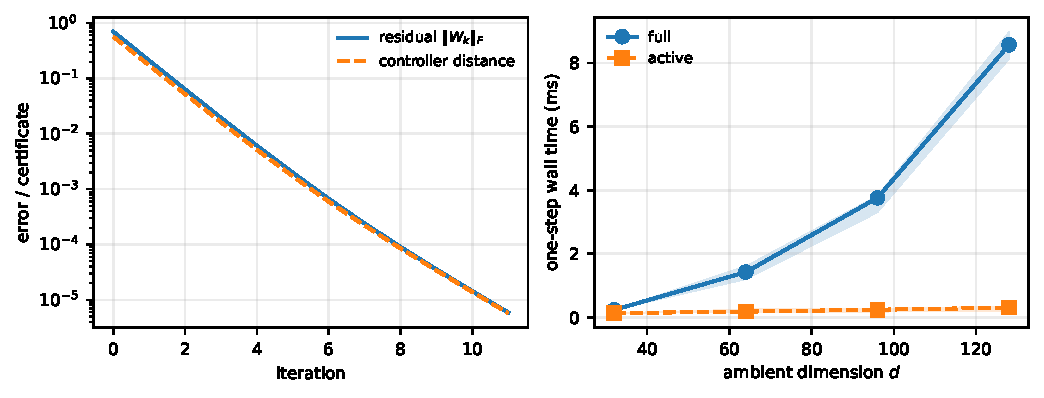
\includegraphics[width=0.94\textwidth]{figures/validation.pdf}
  \caption{Left: residual certificate and reference controller distance for one
  fixed synthetic instance; the other seeds give the same qualitative decay.
  Right: median wall time for one full and active step, with interquartile
  bands over three seeds and seven repetitions after an unmeasured warm-up;
  measurement order is alternated and BLAS uses one thread.  Here \(m=s=4\), so the active
  spectral kernel remains \(r=8\) while \(d\) grows.  Timings are
  implementation and hardware dependent; the invariant result is the kernel
  dimension in \cref{cor:active-core-solver}.}
  \label{fig:validation}
\end{figure}

\paragraph{Dimension and boundary sensitivity.}
We fixed \(m=s=4\) and used ambient dimensions \(32,64,96,128\).  The full
step acts on a dense matrix whose order grows with \(d\), whereas the active
step keeps an order-eight spectral kernel.  At \(d=128\), the observed median one-step times
were \(8.57\) ms and \(0.307\) ms.  The median of the \(21\) paired full/active
time ratios was \(26.9\) in this reference Python implementation.  The
corresponding storage proxies \(d^2\) and
\(dm+r^2\) are \(16384\) and \(576\) scalar entries.

To approach the feasibility boundary, we varied
\(\lambda_{\min}(A^\top B)=\lambda_{\min}(M)\) from \(1\) to \(10^{-3}\)
while holding dimensions and random directions fixed.  Median \(D_0\) grew
from \(0.994\) to \(13.98\), median \(L_0\) from \(1.159\) to \(9.885\), and
the median iterations needed for residual \(10^{-8}\) from \(8\) to \(126\)
(the range over all instances was \(8\)--\(143\)).  Thus the experiment
exposes the rate constant's sensitivity before feasibility is lost; it does
not extrapolate the theorem to singular \(A^\top B\).

\paragraph{Same-objective baseline and nested recovery.}
We also compared the explicit \(1/L_0\) step with a Riemannian gradient method
using Armijo backtracking on the same hidden-coordinate objective and from the
same identity start.  At residual tolerance \(10^{-8}\), median iteration
counts over the three seeds were \(17\) and \(11\), while median objective
evaluations were \(18\) and \(23\), respectively.  Thus line search used fewer
accepted steps but more objective evaluations; the explicit step supplies its
rate and admissibility without backtracking.  This comparison isolates step
selection and does not compare against methods with different feasible models.

Finally, for random \(8\times8\) Hessians we used cumulative ranks
\(2,4,7\) and stopped each inner projection at residual \(10^{-3}\).  Across
three seeds, the largest actual-inner-error/certificate ratio was \(0.983\),
and the largest left/right ratio in
\cref{eq:approximate-multisecant-pythagorean} was
\(1+9.3\times10^{-15}\).  The rank-seven output recovered \(P_\star\) within
\(1.3\times10^{-14}\) AIRM distance; relative cumulative-action error stayed
below \(2.4\times10^{-15}\).  This test evaluates the exact-feasibility model
in floating point and reports the resulting feasibility drift separately.

\begin{figure}[t]
  \centering
  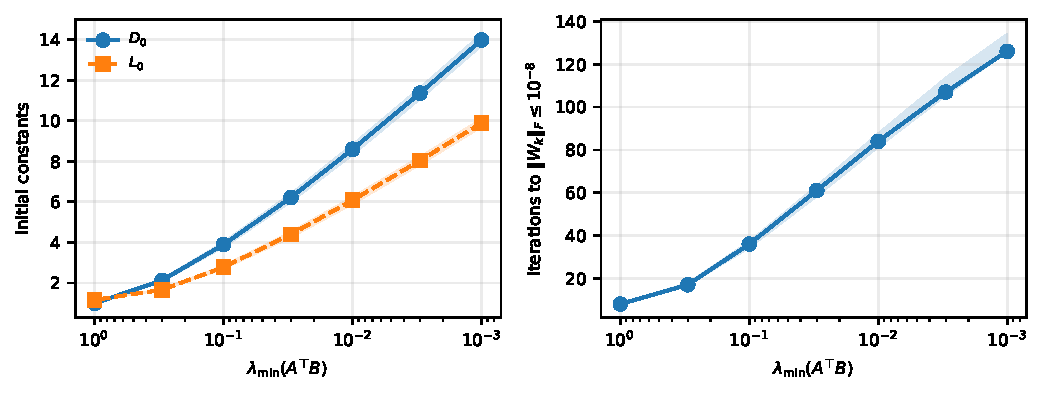
\includegraphics[width=0.94\textwidth]{figures/boundary_sensitivity.pdf}
  \caption{Sensitivity as \(A^\top B\) approaches the positive-definite
  boundary.  Curves show medians and shaded interquartile ranges over the three
  fixed seeds.  Both the analytic radius majorant and the observed iteration
  count deteriorate while every tested instance remains feasible.}
  \label{fig:boundary-sensitivity}
\end{figure}

These experiments test the exact formulas in standard floating point.  They
do not instantiate the certified residual-oracle model of
\cref{cor:inexact-action-solver}; an end-to-end implementation of that model
would require rigorous enclosures for every matrix function and update.

\section{Canonical Multi-Secant Recovery}
\label{sec:multisecant-recovery}

The posterior-certified exact solver computes one canonical action projection.  Nested action
fibers turn those projections into a finite inverse-shape recovery law.  Let
\(H\in\SPD^d\) be a fixed quadratic Hessian and define its determinant-one
inverse shape
\begin{equation}
  P_\star=c_HH^{-1},
  \qquad c_H=(\det H)^{1/d}.
  \label{eq:inverse-shape}
\end{equation}
The scalar \(c_H\) is assumed known, or supplied by an independent scalar
gauge.  This information requirement is part of the theorem.

Let \(S^{(1)},\ldots,S^{(K)}\) have strictly nested column spaces, delete
dependent columns, and write \(r_k=\rank S^{(k)}\).  Define the cumulative
shape-normalized actions
\begin{equation}
  A_k=HS^{(k)},
  \qquad B_k=c_HS^{(k)},
  \qquad
  \mathscr C_k=\{P\in\Pdet:PA_k=B_k\}.
  \label{eq:nested-action-fibers}
\end{equation}
Then \(P_\star\in\mathscr C_k\) and
\(\mathscr C_{k+1}\subset\mathscr C_k\).  Starting from any
\(P_0\in\Pdet\), define
\begin{equation}
  P_k=\argminop_{P\in\mathscr C_k}\dai(P_{k-1},P).
  \label{eq:canonical-multisecant-update}
\end{equation}

\begin{theorem}[Nested canonical multi-secant identification]
\label{thm:nested-multisecant}
For the exact outer projections in \eqref{eq:canonical-multisecant-update},
every update exists uniquely and
preserves all earlier cumulative secants.  For every \(k\),
\begin{equation}
  \boxed{
  \dai(P_k,P_\star)^2+
  \dai(P_{k-1},P_k)^2
  \le\dai(P_{k-1},P_\star)^2.}
  \label{eq:multisecant-pythagorean}
\end{equation}
Consequently,
\begin{align}
  \sum_{j=1}^k\dai(P_{j-1},P_j)^2
  &\le\dai(P_0,P_\star)^2-
       \dai(P_k,P_\star)^2,
  \label{eq:multisecant-energy}\\
  \sum_{j=1}^k\dai(P_{j-1},P_j)
  &\le\sqrt{k}\,\dai(P_0,P_\star).
  \label{eq:multisecant-length}
\end{align}
The determinant-one identification threshold is sharp:
\begin{equation}
  r_K=d-1\quad\Longrightarrow\quad P_K=P_\star,
  \label{eq:sharp-identification-sufficiency}
\end{equation}
whereas any cumulative rank \(r\le d-2\) leaves infinitely many feasible
determinant-one SPD completions.  If each pre-final round contributes exactly
\(b\) new independent probe directions and the final round contributes the
remainder, exact recovery occurs after
\begin{equation}
  K=\left\lceil\frac{d-1}{b}\right\rceil
  \label{eq:block-identification-rounds}
\end{equation}
rounds.  Each exact outer projection reduces by AIRM congruence to the
identity-reference problem in \cref{thm:certified-action-solver}; the inner
iteration converges globally to it and supplies a residual certificate for a
finite approximation.
\end{theorem}

The outer decrease remains quantitative when each projection is stopped after
finitely many certified inner iterations.  Set \(\widetilde P_0=P_0\).  At
round \(k\), let
\[
  Q_k=\operatorname{Proj}_{\mathscr C_k}(\widetilde P_{k-1})
\]
be the exact projection used only for analysis, and let
\(\widetilde P_k\in\mathscr C_k\) be the feasible inner output.  This theorem
uses the exact-feasibility model: action-chart inner iterates lie in
\(\mathscr C_k\) in exact arithmetic.  Floating-point feasibility error is a
separate perturbation and is not included in \(\varepsilon_k\).

\begin{theorem}[Residual-controlled finite inner projections]
\label{thm:approximate-multisecant}
Suppose a posterior inner certificate gives
\begin{equation}
  \dai(\widetilde P_k,Q_k)\le\varepsilon_k.
  \label{eq:inner-projection-certificate}
\end{equation}
Then, with \(D_k=\dai(\widetilde P_k,P_\star)\),
\begin{align}
  &\dai(\widetilde P_{k-1},\widetilde P_k)^2+D_k^2
  \nonumber\\
  &\qquad\le D_{k-1}^2
  +2\sqrt2\,\varepsilon_kD_{k-1}+2\varepsilon_k^2,
  \label{eq:approximate-multisecant-pythagorean}\\
  D_k&\le D_{k-1}+\varepsilon_k
  \le D_0+\sum_{j=1}^k\varepsilon_j.
  \label{eq:approximate-multisecant-distance}
\end{align}
Consequently,
\begin{equation}
  \sum_{j=1}^k
  \dai(\widetilde P_{j-1},\widetilde P_j)^2
  \le D_0^2-D_k^2
  +\sum_{j=1}^k
   \left(2\sqrt2\,\varepsilon_jD_{j-1}+2\varepsilon_j^2\right).
  \label{eq:approximate-multisecant-energy}
\end{equation}
All earlier cumulative actions remain exact because
\(\widetilde P_k\in\mathscr C_k\subseteq\mathscr C_j\) for \(j<k\).
After congruence to the identity-reference inner problem,
\cref{eq:solver-distance-certificate} permits the observable choice
\(\varepsilon_k=\fro{W_{B,k}(\widetilde\Sigma_k)}\); under the residual-oracle
model, \cref{eq:inexact-certificates} supplies the corresponding enlarged
bound.  If \(r_K=d-1\), then \(\mathscr C_K=\{P_\star\}\), so every feasible
inner output at the final round equals \(P_\star\) exactly.
\end{theorem}

The known scalar gauge cannot be dropped.  Ordinary Hessian-vector secants in
\(d-1\) directions do not determine the inverse shape.  In dimension two,
\[
  H_t=\operatorname{diag}(1,t),\qquad s=e_1
\]
gives the same observation \(H_ts=e_1\) for every \(t>0\), while
\[
  (\det H_t)^{1/2}H_t^{-1}
  =\operatorname{diag}(\sqrt t,1/\sqrt t)
\]
varies with \(t\).  Thus \eqref{eq:sharp-identification-sufficiency} is a
sharp theorem for shape-normalized exact actions, rather than a claim of
scale-free identification from ordinary secants.  Acquisition of \(c_H\) is
external to the action oracle and is not claimed to be cheaper than an
additional probe.

\section{Conclusion and Extensions}
\label{sec:discussion}

We studied affine-invariant least-deformation completion from the exact action
\(PA=B\).  The global bundle theorem identifies every determinant-one feasible
fiber and its analytic nearest-controller section.  Total geodesy and the
explicit logarithmic residual turn this geometric selection into a globally
linearly convergent reduced solver with posterior certificates.  From the
identity, or another active-compatible hidden state, the active realization
confines all dense matrix functions to dimension \(r\le2m\); arbitrary hidden
starts retain convergence without this operation bound.  Nested action fibers
further yield exact and residual-controlled approximate Pythagorean decreases
and the sharp rank threshold for normalized inverse-Hessian recovery.

Variational reduction unifies these conclusions.  Its vertical Hessian governs
both response and computation: in Corollary~\ref{cor:action-interaction-response},
\(H_B^{-1}\) maps mechanism
perturbations to interaction curvature and visible-action perturbations to
canonical-section susceptibility.  For the unperturbed completion problem,
the same fiber geometry produces the optimization residual and its
certificates.  The resulting chain is
\[
  \begin{aligned}
    \text{reduction}
    &\;\longrightarrow\;\text{vertical response}
      \;\longrightarrow\;\text{action bundle}\\
    &\;\longrightarrow\;\text{posterior-certified active solver}.
  \end{aligned}
\]

The controlled experiments reproduce the posterior inequalities, exact
full--active trajectory equivalence to numerical precision, and the fixed-size
active spectral kernel as \(d\) grows.  They also show increasing initial
radius, curvature majorant, and iteration count as \(A^\top B\) approaches the
positive-definite boundary.  This is a conditioning diagnostic, not an
analytic boundary-rate theorem.

Several extensions arise directly from the formulation.  An end-to-end
finite-precision implementation must supplement the residual-oracle theorem
with certified exponential updates, factorizations, active bases, determinant
maintenance, and stored iterates; combining those enclosures with the present
spectral-arithmetic count would yield a bit-complexity result.  The recovery
law can be extended by treating the determinant gauge as an additional unknown
or observation.  Structured controller families replace the totally geodesic
full-SPD fiber by a restricted feasible set, while noisy actions replace exact
completion by statistical or robust projection.  These variants provide the
route from exact canonical completion to implementable adaptive
preconditioners.

\section*{Data and Code Availability}

The deterministic synthetic generator, full and active reference
implementations, fixed configuration, raw CSV results, and figure-generation
script are included in the source archive under \texttt{experiments/}.  They
use no external datasets.  Seeds, dimensions, tolerances, repetitions, and
software requirements are recorded in \texttt{experiments/config.json} and
\texttt{experiments/README.md}.  The code evaluates the exact-arithmetic
formulas with standard floating-point eigendecompositions; it is numerical
validation, not a certified matrix-function package.  The residual-oracle
result still assumes rigorous direction-error and initial-radius majorants
satisfying \cref{eq:computable-relative-error-test}, and its implementation
boundary is stated after \cref{cor:inexact-action-solver}.


\bibliographystyle{tmlr}
\bibliography{references}

\appendix
\section{Proofs for Variational Reduction and Response}
\label{app:reduction-response}

\subsection{Algebraic reduction}

\begin{proof}[Proof of \cref{thm:algebraic-reduction}]
Fix \(z\in\Zspace\).  Partitioning the composite fiber by its intermediate
visible value gives
\[
\begin{aligned}
  ((\rho\circ\pi)_!E)(z)
  &=\inf_{x:\rho(\pi(x))=z}E(x)\\
  &=\inf_{y:\rho(y)=z}\inf_{x:\pi(x)=y}E(x)\\
  &=(\rho_!(\pi_!E))(z).
\end{aligned}
\]
Likewise,
\[
\begin{aligned}
  \inf_x\{E(x)+\ell(\pi(x))\}
  &=\inf_y\inf_{\pi(x)=y}\{E(x)+\ell(y)\}\\
  &=\inf_y\{(\pi_!E)(y)+\ell(y)\}.
\end{aligned}
\]
The base-potential law follows because \(\varphi(\pi(x))=\varphi(y)\) is
constant on each fiber.  The constraint law follows from the definition of
the indicator energy.  No attainment assumption is used.
\end{proof}

\subsection{Existence and uniqueness of the canonical lift}

\begin{proof}[Proof of \cref{thm:canonical-lift}]
Fix \(y\) with finite reduced energy.  Coercivity places every minimizing
sequence in a bounded sublevel set.  Properness makes its closure compact, and
lower semicontinuity gives a minimizer in the closed fiber.

If \(x_0\ne x_1\) were two minimizers, their fiber geodesic would satisfy
\[
  E(x_0\#_{1/2}x_1)
  \le\frac12E(x_0)+\frac12E(x_1)
  -\frac\mu8d(x_0,x_1)^2,
\]
contradicting minimality.  Thus the minimizer is unique.

For equivariance, \(g s_E(y)\) lies in the fiber over \(gy\) and has the same
energy as \(s_E(y)\).  Uniqueness on that fiber gives
\(s_E(gy)=g s_E(y)\).
\end{proof}

\subsection{Smooth minimizer response}

\begin{proof}[Proof of \cref{thm:response-schur}]
We first show continuity of the global minimizer section.  Let \(z_k\to z\).
Choose one fixed trial point near \(\sigma_\star(z)\).  Continuity of \(E\)
uniformly bounds the optimal values for all sufficiently large \(k\).  Local
uniform inf-compactness therefore places \(\sigma_\star(z_k)\) in a common
relatively compact set.  Every convergent subsequence has a limit
\(\bar\sigma\).  Optimality and continuity give, for every trial \(\sigma\),
\[
  E(z,\bar\sigma)
  =\lim E(z_k,\sigma_\star(z_k))
  \le\lim E(z_k,\sigma)=E(z,\sigma).
\]
The minimizer at \(z\) is unique, so \(\bar\sigma=\sigma_\star(z)\).  Every
subsequence has the same limit, proving continuity.

The first-order condition is
\begin{equation}
  E_\sigma(z,\sigma_\star(z))=0.
  \label{eq:appendix-stationarity}
\end{equation}
Its derivative with respect to \(\sigma\) is the invertible matrix \(H\).
The implicit-function theorem gives a local \(C^r\) critical section.  The
continuous global minimizer section agrees with it near every point and is
therefore \(C^r\).  Differentiating
\cref{eq:appendix-stationarity} gives
\[
  E_{\sigma z}+H D_z\sigma_\star=0,
\]
which proves \cref{eq:hidden-response}.  The chain rule gives
\[
  D_z\bar E
  =E_z+E_\sigma D_z\sigma_\star=E_z,
\]
and a second derivative gives
\[
  D^2_{zz}\bar E
  =E_{zz}+E_{z\sigma}D_z\sigma_\star
  =E_{zz}-E_{z\sigma}H^{-1}E_{\sigma z}.
\]

For nested variables \(\sigma=(\alpha,\beta)\), let \(q\) be the quadratic
form defined by the complete Hessian at the optimum.  Positive definiteness of
the joint hidden block makes both quadratic minimizations unique.  Algebraic
reduction gives
\[
  \inf_{\delta\alpha,\delta\beta}
  q(\delta z,\delta\alpha,\delta\beta)
  =\inf_{\delta\alpha}
  \left(\inf_{\delta\beta}
  q(\delta z,\delta\alpha,\delta\beta)\right).
\]
The matrix of a partially minimized quadratic form is the corresponding Schur
complement.  Equality for every \(\delta z\) proves
\cref{eq:schur-associativity}.
\end{proof}

\subsection{Interaction curvature and finite contrasts}

\begin{proof}[Proof of \cref{thm:interaction-curvature}]
For \cref{eq:affine-interventions},
\[
  E_{uu}=0,
  \qquad
  E_{\sigma u}=G.
\]
The \(u\)-block of \cref{eq:schur-effective-hessian} is therefore
\[
  D^2_{uu}\bar E=-G^*H^{-1}G.
\]
For every \(a\in\mathbb R^p\),
\[
  \ip{a}{D^2_{uu}\bar E\,a}
  =-\ip{Ga}{H^{-1}Ga}\le0,
\]
because \(H^{-1}\succ0\).  Expanding in coordinate vectors gives
\cref{eq:pair-interaction-curvature}.  A mixed entry is zero exactly when the
two corresponding covectors are orthogonal under the inner product induced by
\(H^{-1}\).  Finally, without differentiability,
\[
  \bar E(y,u)=\inf_\sigma
  \left(E_0(y,\sigma)+\sum_i u_i\Delta_i(y,\sigma)\right)
\]
is a pointwise infimum of affine functions of \(u\), hence concave.
\end{proof}

\subsection{Finite contrasts and order of reduction}
\label{app:finite-contrasts}

\begin{corollary}[Factorial finite differences]
\label{cor:factorial-contrast}
Assume \([0,1]^p\subset\Uspace\).  For \(T\subseteq[p]\), define
\begin{equation}
  \delta_T\bar E
  =\sum_{B\subseteq T}(-1)^{|T|-|B|}
  \bar E(y,\mathbf1_B).
  \label{eq:factorial-contrast}
\end{equation}
If \(\bar E\in C^{|T|}\), then
\begin{equation}
  \delta_T\bar E
  =\int_{[0,1]^T}
  \partial_T^{|T|}\bar E(u_T,0_{T^c})\,\dd u_T.
  \label{eq:factorial-integral}
\end{equation}
\end{corollary}

\begin{proof}
For a single coordinate, the fundamental theorem of calculus gives
\[
  \bar E(e_i)-\bar E(0)
  =\int_0^1\partial_{u_i}\bar E(t e_i)\,\dd t.
\]
Apply the same identity successively to each coordinate in \(T\).  The product
of difference operators expands as
\[
  \prod_{i\in T}(\mathsf T_i-I)\bar E(0)
  =\sum_{B\subseteq T}(-1)^{|T|-|B|}\bar E(\mathbf1_B),
\]
and repeated integration gives
\[
  \prod_{i\in T}(\mathsf T_i-I)\bar E(0)
  =\int_{[0,1]^T}\partial_T^{|T|}\bar E(u_T,0_{T^c})\,\dd u_T.
\]
For \(T=\{i,j\}\), substitute
\cref{eq:pair-interaction-curvature} to obtain
\cref{eq:pair-factorial-integral}.
\end{proof}

Reduction need not commute with finite differencing.  For
\[
  E_0(\sigma)=\sigma^2,\qquad E_1(\sigma)=(\sigma-1)^2,
\]
both reduced minima are zero, but
\(\inf_\sigma(E_1-E_0)=\inf_\sigma(1-2\sigma)=-\infty\).
Thus hidden states must be reduced first.  If every perturbation
\(\Delta_i\) is constant on each fiber, the minimizer is unchanged and all
higher-order contrasts vanish; this is the exact commuting case.

\section{Proof of the Global SPD Action Bundle}
\label{app:action-bundle}

\begin{proof}[Proof of \cref{thm:action-bundle}]
We proceed in seven steps.

\paragraph{Step 1: coordinates on the action base.}
Put \(Y=BC^{-1}\).  Since \(Q=[U,V]\) is orthogonal,
\[
  Y=UM+VN,
  \qquad M=U^\top Y,
  \qquad N=V^\top Y.
\]
Moreover,
\[
  A^\top B=C^\top M C,
\]
so \(A^\top B\in\SPD^m\) exactly when \(M\in\SPD^m\).  The map
\(B\mapsto(M,N)\) has the analytic inverse
\begin{equation}
  B=(UM+VN)C.
  \label{eq:appendix-base-inverse}
\end{equation}
Thus \(\Bact\cong\SPD^m\times\mathbb R^{n\times m}\).

\paragraph{Step 2: every SPD completion.}
Suppose \(P\in\SPD^d\) satisfies \(PA=B\).  Because \(A=UC\), this is
equivalent to \(PU=Y\).  In the \(Q\) coordinates, symmetry fixes the first
block row and column:
\[
  \widehat P:=Q^\top P Q
  =\begin{pmatrix}M&N^\top\\N&D\end{pmatrix}.
\]
The Schur-complement criterion gives
\[
  \widehat P\succ0
  \quad\Longleftrightarrow\quad
  S:=D-NM^{-1}N^\top\succ0.
\]
With \(T=NM^{-1}\), every positive solution and only such a solution is
\begin{equation}
  \widehat P
  =L\begin{pmatrix}M&0\\0&S\end{pmatrix}L^\top.
  \label{eq:appendix-all-completions}
\end{equation}
Since \(\det L=1\),
\[
  \det P=\det M\det S.
\]
The determinant-one constraint is therefore equivalent to
\[
  S=\rho\Sigma,
  \qquad \rho=(\det M)^{-1/n},
  \qquad \det\Sigma=1,
\]
which is exactly \cref{eq:action-bundle-map}.  Conversely, direct block
multiplication and \cref{eq:appendix-base-inverse} give
\[
  \Phi_A(B,\Sigma)A
  =Q\begin{pmatrix}M\\N\end{pmatrix}C=B.
\]

\paragraph{Step 3: analytic inverse.}
Given \(P\in\Pdet\), recover \(B=PA\), then \(M(B),N(B)\), and the unique
Schur complement
\[
  S=D-NM^{-1}N^\top.
\]
The unique determinant-one hidden coordinate is
\begin{equation}
  \Sigma=(\det M)^{1/n}S.
  \label{eq:appendix-hidden-inverse}
\end{equation}
All operations are analytic on their SPD domains.  Thus \(\Phi_A\) is a
global analytic diffeomorphism and \(\pi_A\) is projection onto its first
factor.

\paragraph{Step 4: fiber geometry.}
Fix \(B\).  Before congruence by \(QL\), the fiber is
\[
  \mathcal C_B
  =\{\operatorname{diag}(M,\rho\Sigma):\Sigma\in\mathscr P_n\}.
\]
The ambient AIRM geodesic between two such points is
\[
  \operatorname{diag}(M,\rho\Sigma_0)
  \#_t
  \operatorname{diag}(M,\rho\Sigma_1)
  =\operatorname{diag}(M,\rho(\Sigma_0\#_t\Sigma_1)).
\]
Because log determinant is affine along AIRM geodesics,
\(\det(\Sigma_0\#_t\Sigma_1)=1\).  Hence the fiber is totally geodesic.
It is closed, and block distance splitting gives
\[
  \dai(\operatorname{diag}(M,\rho\Sigma_0),
       \operatorname{diag}(M,\rho\Sigma_1))
  =\dai(\Sigma_0,\Sigma_1).
\]
Congruence by \(QL\) is an AIRM isometry, proving all fiber claims.

\paragraph{Step 5: canonical projection and analyticity.}
The determinant-one SPD slice is a finite-dimensional Hadamard manifold.  A
nonempty closed geodesically convex set has a unique metric projection, so
\cref{eq:canonical-controller} defines a global section.

In the global coordinates define
\[
  F(B,\Sigma)=\frac12\fro{\log\Phi_A(B,\Sigma)}^2.
\]
This function is analytic.  For fixed \(B\), its hidden variable parameterizes
an isometric totally geodesic fiber.  Squared distance to \(I\), restricted to
that fiber, is strongly geodesically convex.  At the unique critical point the
vertical Hessian is positive definite.  The analytic implicit-function theorem
therefore gives a local analytic minimizer \(\Sigma_\star(B)\); global
uniqueness makes these local sections agree.  Hence
\[
  s_A(B)=\Phi_A(B,\Sigma_\star(B))
\]
and \(\mathfrak C_A(B)^2=2F(B,\Sigma_\star(B))\) are analytic.

\paragraph{Step 6: equivariance.}
For \(D\in\operatorname{GL}_m\),
\[
  P(AD)=BD\quad\Longleftrightarrow\quad PA=B,
\]
so the two action fibers are identical and have the same unique projection.
For \(R\in O(d)\),
\[
  PA=B
  \quad\Longleftrightarrow\quad
  (RPR^\top)(RA)=RB.
\]
Orthogonal congruence preserves determinant and distance to \(I\), so
uniqueness gives \cref{eq:controller-equivariance}.

\paragraph{Step 7: normal equation and certificate.}
Congruence invariance reduces the hidden objective to
\[
  f_B(\Sigma)=\frac12\dai(R_0,\mathcal Q_\Sigma)^2.
\]
We use the convention that a function is \(1\)-strongly geodesically convex
when every constant-speed geodesic \(\gamma_t\) satisfies
\begin{equation}
  f(\gamma_t)
  \le (1-t)f(\gamma_0)+t f(\gamma_1)
  -\frac12t(1-t)d(\gamma_0,\gamma_1)^2.
  \label{eq:cat0-strong-convexity-convention}
\end{equation}
On a CAT(0) space this inequality holds for
\(f(\cdot)=\tfrac12d(\cdot,R_0)^2\).  The AIRM SPD manifold is Hadamard, and
restriction to the isometric totally geodesic determinant-one fiber preserves
the same constant \cite{bhatia2007positive,lim2004best}.
A whitened tangent to the determinant-one hidden block has the form
\[
  Z=\begin{pmatrix}0&0\\0&Z_{22}\end{pmatrix},
  \qquad Z_{22}=Z_{22}^\top,
  \qquad \tr Z_{22}=0.
\]
The whitened negative gradient is the tangent projection of
\(\mathcal R(\Sigma)\) in \cref{eq:action-residual}.  Orthogonality to every
trace-free \(Z_{22}\) is exactly
\(\mathcal R_{22}(\Sigma)^\circ=0\).  Strong convexity makes this condition
necessary and sufficient.

Let \(D=\dai(\Sigma,\Sigma_\star)\), let
\(\xi=\operatorname{Log}_\Sigma(\Sigma_\star)\), and let \(V(\Sigma)\) be the restricted
negative gradient.  The first-order form of
\cref{eq:cat0-strong-convexity-convention} gives
\[
  f_B(\Sigma)-f_B(\Sigma_\star)
  \le \langle V(\Sigma),\xi\rangle-\frac12D^2
  \le\norm{V(\Sigma)}D-\frac12D^2,
\]
while the same inequality based at the minimizer, whose gradient vanishes,
gives
\[
  f_B(\Sigma)-f_B(\Sigma_\star)\ge\frac12D^2.
\]
Adding the two bounds yields
\[
  D^2\le\norm{V(\Sigma)}D,
\]
and hence, also for \(D=0\),
\[
  D\le\norm{V(\Sigma)}
  =\fro{\mathcal R_{22}(\Sigma)^\circ}.
\]
Finally,
\[
  f_B(\Sigma)-f_B(\Sigma_\star)
  \le \sup_{D\ge0}
  \left(\norm{V(\Sigma)}D-\frac12D^2\right)
  =\frac12\norm{V(\Sigma)}^2.
\]
This proves the exact constants in
\cref{eq:action-distance-certificate,eq:action-value-certificate}.
\end{proof}

\subsection{Proof of active reduction}

Let \(J\) be the orthogonal reflection that equals \(+I\) on \(W\) and
\(-I\) on \(W^\perp\).  Since the columns of \(A\) and \(B\) lie in \(W\),
\[
  JA=A,
  \qquad JB=B.
\]
If \(P\in\Pfiber(B)\), then \((JPJ)A=B\), and \(JPJ\) has the same
determinant and distance from \(I\) as \(P\).  Uniqueness of the canonical
controller yields
\[
  Js_A(B)J=s_A(B).
\]
Hence the cross blocks between \(W\) and \(W^\perp\) vanish:
\(s_A(B)=H_\star\oplus C_\star\).

For fixed feasible \(H\), the inactive log-eigenvalues \(z_i\) satisfy
\[
  \sum_{i=1}^qz_i=-\log\det H.
\]
Cauchy--Schwarz gives
\[
  \fro{\log C}^2=\sum_i z_i^2
  \ge\frac{(\log\det H)^2}{q},
\]
with equality exactly when all \(z_i\) are equal.  Thus
\[
  C_\star=(\det H_\star)^{-1/q}I_q,
\]
and substitution yields \cref{eq:active-controller-problem}.  Uniqueness
follows from uniqueness of \(s_A(B)\).

\section{Proofs for the Solver, Certificates, and Recovery Laws}
\label{app:solver-recovery-proofs}

This appendix proves the algorithmic and recovery results in
\cref{sec:certified-solver,sec:multisecant-recovery}.
All gradients, exponential maps, and norms below
use the affine-invariant metric.

\subsection{Curvature and squared-distance comparison}

\begin{lemma}[AIRM curvature bound]
\label{lem:airm-curvature-bound}
Every sectional curvature of \(\SPD^d\), its determinant-one slice
\(\Pdet\), and every action fiber \(\Pfiber(B)\) lies in
\begin{equation}
  -\frac12\le \operatorname{sec}\le0.
  \label{eq:airm-curvature-bound}
\end{equation}
\end{lemma}

\begin{proof}
Congruence invariance reduces the calculation to the identity, where tangent
vectors are symmetric matrices and the metric is Frobenius.  The AIRM
curvature tensor is
\[
  R(X,Y)Z=-\frac14[[X,Y],Z],
\]
and hence
\[
  \operatorname{sec}(X,Y)
  =-\frac14\frac{\fro{[X,Y]}^2}
  {\fro X^2\fro Y^2-\ip X Y_F^2}\le0.
\]
To obtain the lower bound, replace \(Y\) by its component
\(\widetilde Y\) Frobenius-orthogonal to \(X\); this leaves the commutator
unchanged and turns the denominator into
\(\fro X^2\fro{\widetilde Y}^2\).  Orthogonally diagonalize
\(X=\operatorname{diag}(\lambda_i)\).  For symmetric
\(\widetilde Y=(y_{ij})\),
\[
\begin{aligned}
  \fro{[X,\widetilde Y]}^2
  &=2\sum_{i<j}(\lambda_i-\lambda_j)^2y_{ij}^2\\
  &\le4\fro X^2\sum_{i<j}y_{ij}^2
  \le2\fro X^2\fro{\widetilde Y}^2.
\end{aligned}
\]
Substitution gives \(\operatorname{sec}\ge-1/2\).  The determinant-one
slice and the action fibers are totally geodesic, so their intrinsic
curvatures are restrictions of the ambient curvature tensor.
\end{proof}

\begin{lemma}[Squared-distance Hessian comparison]
\label{lem:squared-distance-comparison}
Let \((\mathcal M,g)\) be a finite-dimensional Hadamard manifold with
\(-\kappa\le\operatorname{sec}\le0\).  For fixed \(z\), let
\(h(x)=\tfrac12d(z,x)^2\).  Then
\begin{equation}
  g_x\preceq\operatorname{Hess}h(x)
  \preceq\psi(\sqrt\kappa R)g_x
  \quad\text{whenever }d(z,x)\le R,
  \label{eq:squared-distance-comparison}
\end{equation}
where \(\psi(s)=s\coth s\) and \(\psi(0)=1\).  In particular, \(h\) is
globally \(1\)-strongly geodesically convex.
\end{lemma}

\begin{proof}
For \(x\ne z\), put \(r=d(z,x)\), let \(T\) be the terminal unit tangent
of the geodesic from \(z\) to \(x\), and decompose
\(v=aT+v_\perp\).  The radial Hessian formula gives
\[
  \operatorname{Hess}h(v,v)
  =a^2+r\operatorname{Hess}r(v_\perp,v_\perp).
\]
Let \(J\) be the Jacobi field with \(J(0)=0\) and
\(J(r)=v_\perp\).  Nonpositive curvature and Cauchy--Schwarz applied after
parallel transport yield
\[
  \operatorname{Hess}r(v_\perp,v_\perp)=I(J,J)
  \ge\int_0^r\norm{D_tJ}^2\,\dd t
  \ge r^{-1}\norm{v_\perp}^2.
\]
For the reverse bound, compare \(J\) with
\[
  V(t)=\frac{\sinh(\sqrt\kappa t)}
  {\sinh(\sqrt\kappa r)}P_tv_\perp,
\]
using \(V(t)=(t/r)P_tv_\perp\) when \(\kappa=0\).  The index lemma and the
curvature lower bound give
\[
  I(J,J)\le I(V,V)
  \le\sqrt\kappa\coth(\sqrt\kappa r)\norm{v_\perp}^2.
\]
Therefore
\[
  \norm v^2\le\operatorname{Hess}h(v,v)
  \le\psi(\sqrt\kappa r)\norm v^2.
\]
The formula extends continuously to \(x=z\), where
\(\operatorname{Hess}h=g_z\).  Monotonicity of \(\psi\) proves the stated
radius bound, and integration of the lower Hessian bound along geodesics
proves strong convexity.
\end{proof}

\begin{proof}[Proof of \cref{thm:canonical-fiber-engine}]
Coercivity and closedness give a minimizer, and strong convexity makes it
unique.  Write \(G_k=\operatorname{grad}F(x_k)\),
\(g_k=\norm{G_k}\), and
\[
  \gamma_k(t)=\operatorname{Exp}_{x_k}(-tG_k),
  \qquad 0\le t\le L_0^{-1}.
\]
If \(g_k=0\), strong convexity gives \(x_k=x_\star\).  Otherwise
\((F\circ\gamma_k)'(0)=-g_k^2<0\).  If this update segment left the current
sublevel, continuity would give a first return
\(t_\star\in(0,L_0^{-1}]\).  Before that return the Hessian is bounded by
\(L_0g\), so the integral Taylor formula would give
\[
\begin{aligned}
  F(\gamma_k(t_\star))
  &\le F(x_k)-t_\star g_k^2
       +\frac{L_0t_\star^2}{2}g_k^2\\
  &\le F(x_k)-\frac{t_\star}{2}g_k^2<F(x_k),
\end{aligned}
\]
contradicting the return.  Hence the complete update stays in the current
sublevel, and the same inequality at \(t=L_0^{-1}\) gives
\[
  F(x_{k+1})\le F(x_k)-\frac{g_k^2}{2L_0}.
\]

Let \(\Delta(x)=F(x)-F(x_\star)\),
\(d=d(x,x_\star)\), and
\(g=\norm{\operatorname{grad}F(x)}\).  Strong convexity at \(x\) and at
\(x_\star\) gives
\[
  \frac{\mu}{2}d^2
  \le\Delta(x)
  \le gd-\frac{\mu}{2}d^2
  \le\frac{g^2}{2\mu}.
\]
The first two expressions also imply \(d\le g/\mu\).  Thus
\(g^2\ge2\mu\Delta\), and the descent inequality yields
\[
  \Delta_{k+1}
  \le\left(1-\frac{\mu}{L_0}\right)\Delta_k.
\]
Iteration proves the value rate; the two preceding inequalities prove the
distance and posterior bounds.  Since
\(g_k^2/(2L_0)\le\Delta_k\), they also give the gradient rate.  Exact
inversion of \(q_{\mu,L}^k\) gives the stated complexity.  If
\(L_0=\mu\), the recurrence gives \(\Delta_1=0\).

For \(F(x)=\mu\|x\|^2/2\) on a Euclidean line, both posterior inequalities
and the \(L_0=\mu\) one-step statement hold with equality.
\end{proof}

For the fiber objective \(F_B(P)=\tfrac12\dai(I,P)^2\),
\cref{lem:airm-curvature-bound,lem:squared-distance-comparison} imply
\begin{equation}
  \operatorname{Hess}F_B\succeq g,
  \qquad
  \operatorname{Hess}F_B(P)\preceq
  \psi(D/\sqrt2)g_P
  \quad\text{if }\dai(I,P)\le D.
  \label{eq:fiber-hessian-bounds}
\end{equation}
The following action instance proves that the constant cannot be decreased
uniformly over dimensions and admissible actions.

\begin{proposition}[Action-family attainment of the radius majorant]
\label{prop:sharp-action-majorant}
Let \(d=3\), \(m=1\), and \(A=B=e_1\).  The action fiber is
\[
  \{\operatorname{diag}(1,\Sigma):\Sigma\in\mathscr P_2\},
\]
its canonical controller is \(I_3\), and for every \(D>0\) there are a point
at AIRM radius \(D\) and a unit fiber tangent \(v\) such that
\begin{equation}
  \operatorname{Hess}F_B(v,v)=\psi(D/\sqrt2).
  \label{eq:sharp-action-majorant-attainment}
\end{equation}
Hence \(\psi(D/\sqrt2)\) is the sharp dimension-uniform radius-only Hessian
majorant within the action family.  Along a radial geodesic in the same fiber,
both posterior inequalities in
\cref{eq:solver-distance-certificate,eq:solver-gap-certificate} hold with
equality.
\end{proposition}

\begin{proof}
Here \(M=1\), \(N=0\), and \(\rho=1\), so the displayed fiber and canonical
controller follow directly from \cref{eq:action-bundle-map}.  The
determinant-one surface \(\mathscr P_2\) is a two-dimensional space of
constant sectional curvature \(-1/2\), as equality holds in the commutator
bound of \cref{lem:airm-curvature-bound}.  On a constant-curvature
\(-\kappa\) plane, the transverse eigenvalue of the Hessian of
\(\tfrac12d(I,\cdot)^2\) at radius \(D\) is
\(D\sqrt\kappa\coth(D\sqrt\kappa)\).  Taking \(\kappa=1/2\) gives
\eqref{eq:sharp-action-majorant-attainment}.
\end{proof}

\subsection{Residual gradient and exact global convergence}

\begin{proof}[Proof of \cref{eq:residual-gradient-identity}]
On the ambient SPD manifold, for
\(\widetilde f(Q)=\tfrac12\dai(R_0,Q)^2\),
\[
  -\operatorname{grad}\widetilde f(Q)=\operatorname{Log}_Q(R_0).
\]
Whitening at \(Q\) turns this tangent into
\(\log(Q^{-1/2}R_0Q^{-1/2})\).  At
\(Q=\mathcal Q_\Sigma\) it is precisely \(\mathcal R(\Sigma)\).
The whitened tangent space of the hidden determinant-one block consists of
\[
  \begin{pmatrix}0&0\\0&Z\end{pmatrix},
  \qquad Z=Z^\top,\quad\tr Z=0.
\]
Since whitening converts the AIRM inner product to the Frobenius inner
product, orthogonal projection retains the \(22\) block and removes its
trace.  Thus the whitened reduced negative gradient is
\(W_B(\Sigma)=\mathcal R_{22}(\Sigma)^\circ\), which proves both identities
in \cref{eq:residual-gradient-identity}.
\end{proof}

\begin{proof}[Proof of \cref{thm:certified-action-solver}]
Set
\[
  f_k=f_B(\Sigma_k),\qquad
  g_k=\fro{W_B(\Sigma_k)},\qquad
  D_k=\dai(R_0,\mathcal Q_{\Sigma_k})=\sqrt{2f_k}.
\]
Trace freeness of
\(W_B(\Sigma_k)\) preserves determinant one, while the exponential preserves
positive definiteness.  The action chart consequently keeps every controller
on \(\Pfiber(B)\).

Let \(\gamma_k(t)\) be the negative-gradient geodesic, parameterized for
\(0\le t\le L_0^{-1}\), and put
\(\varphi_k=f_B\circ\gamma_k\).  If \(g_k=0\), the iterate is optimal.
Otherwise \(\varphi_k'(0)=-g_k^2<0\).  If the update segment left the
current objective sublevel, there would be a first return
\(t_\star\in(0,L_0^{-1}]\).  Before that return,
\(D(\gamma_k(t))\le D_k\le D_0\), so
\eqref{eq:fiber-hessian-bounds} bounds the Hessian by \(L_0g\).  The
integral Taylor formula would then imply
\[
  \varphi_k(t_\star)
  \le\varphi_k(0)-t_\star g_k^2
      +\frac{L_0t_\star^2}{2}g_k^2
  <\varphi_k(0),
\]
a contradiction.  Thus the complete update segment stays in the current
sublevel.  Applying the same Taylor bound at \(L_0^{-1}\) gives
\[
  f_{k+1}\le f_k-\frac1{L_0}g_k^2
  +\frac1{2L_0}g_k^2
  =f_k-\frac1{2L_0}g_k^2.
\]
Thus \(D_{k+1}\le D_k\), closing the induction and proving
\cref{eq:solver-descent} globally.

Let \(\Delta(\Sigma)=f_B(\Sigma)-f_B(\Sigma_\star)\).  Strong convexity
and Cauchy--Schwarz give, with
\(d=\dai(\Sigma,\Sigma_\star)\) and
\(g=\norm{\operatorname{grad}f_B(\Sigma)}\),
\begin{equation}
  \Delta(\Sigma)\le gd-\frac12d^2\le\frac12g^2.
  \label{eq:proof-pl}
\end{equation}
Hence \(g^2\ge2\Delta\), and the descent inequality yields
\[
  \Delta_{k+1}\le(1-L_0^{-1})\Delta_k=q_0\Delta_k.
\]
Since \(\Delta_0\le f_0=D_0^2/2\), this proves
\cref{eq:solver-value-rate}.  Strong convexity based at the minimizer gives
\(d^2\le2\Delta\), proving \cref{eq:solver-distance-rate}.  Combining
\(f_{k+1}\ge f_B(\Sigma_\star)\) with the descent inequality gives
\(g_k^2\le2L_0\Delta_k\), proving
\cref{eq:solver-residual-rate}.

The two strong-convexity inequalities also give
\(\Delta\ge d^2/2\).  Together with the first bound in
\eqref{eq:proof-pl}, this implies \(d\le g\), including the case \(d=0\),
while the second bound in \eqref{eq:proof-pl} gives
\(\Delta\le g^2/2\).  These are
\cref{eq:solver-distance-certificate,eq:solver-gap-certificate}.
Finally, for \(D_0>0\),
\(q_0^k=e^{-k\chi_0}\).  Solving the three rate bounds exactly for \(k\)
gives
\cref{eq:solver-value-complexity,eq:solver-distance-complexity,eq:solver-residual-complexity}.
The case \(D_0=0\) is immediate.
\end{proof}

\subsection{Active and inexact implementations}

\begin{proof}[Proof of \cref{cor:active-core-solver}]
Retain \(A=UC\) from \cref{sec:action-bundle}.  Choose \(V_a\) so that
\(E=[U,V_a]\) is an orthonormal basis of \(\mathcal W_A\).  Then
\[
  BC^{-1}=UM+V_aN_a,\qquad
  T_a=N_aM^{-1},\qquad
  L_a=\begin{pmatrix}I&0\\T_a&I\end{pmatrix},
  \qquad
  R_{0,a}=L_a^{-1}L_a^{-\top}.
\]
Complete \(E\) by \(Z\) when \(q>0\).  In the basis \([U,V_a,Z]\), the
full action coordinate satisfies
\[
  N=\begin{pmatrix}N_a\\0\end{pmatrix},
  \qquad
  L=L_a\oplus I_q,
  \qquad
  R_0=R_{0,a}\oplus I_q.
\]
An active-compatible initializer has the form
\[
  \Sigma=\Sigma_a\oplus\beta I_q,
  \qquad
  \det\Sigma_a\,\beta^q=1.
\]
The identity default corresponds to \(\Sigma_a=I_s\) and \(\beta=1\).
Then
\[
  \mathcal Q_a=\operatorname{diag}(M,\rho\Sigma_a),
  \qquad
  \mathcal Q_\Sigma
  =\mathcal Q_a\oplus(\rho\beta)I_q,
\]
and block functional calculus gives
\[
  \mathcal R_a
  =\log(\mathcal Q_a^{-1/2}R_{0,a}\mathcal Q_a^{-1/2}),
  \qquad
  \mathcal R(\Sigma)
  =\mathcal R_a\oplus r_cI_q,
  \qquad
  r_c=-\log(\rho\beta).
\]
The hidden trace-free projection subtracts the common mean
\[
  \tau=\frac{\tr\mathcal R_{22}^a+qr_c}{s+q}.
\]
Consequently,
\begin{equation}
  \begin{aligned}
    W_B(\Sigma)&=W_a\oplus w_cI_q,
    &W_a&=\mathcal R_{22}^a-\tau I_s,
    &w_c&=r_c-\tau,\\
    \fro{W_B(\Sigma)}^2&=\fro{W_a}^2+qw_c^2.
  \end{aligned}
\label{eq:active-residual-splitting}
\end{equation}
The full exponential update now splits exactly into
\begin{equation}
  \Sigma_a^+
  =\Sigma_a^{1/2}e^{W_a/L_0}\Sigma_a^{1/2},
  \qquad
  \beta^+=\beta e^{w_c/L_0}.
\label{eq:active-solver-update-proof}
\end{equation}
Since \(\tr W_a+qw_c=0\), this update preserves
\(\det\Sigma_a\,\beta^q=1\).  The action-bundle map then preserves
positive definiteness, determinant one, and \(PA=B\).  This proves
\eqref{eq:active-residual-splitting} and
\eqref{eq:active-solver-update-proof}; the
stopping certificate follows from
\cref{eq:solver-distance-certificate}.

A rank-revealing thin QR of the \(d\times2m\) input costs \(O(dm^2)\).
All remaining preprocessing acts on matrices of order at most \(r\), costing
\(O(r^3)\).  Each iteration uses one \(r\times r\) logarithm and inverse
square root and one \(s\times s\) exponential, hence \(O(r^3)\) arithmetic
and \(O(r^2)\) working memory.  Combining this cost with
\cref{eq:solver-residual-complexity} gives
\cref{eq:active-total-complexity}.  The representation
\[
  Px=cx+E(H-cI_r)E^\top x
\]
costs \(O(dr+r^2)\) per application.  If \(q=0\), every complement term is
absent and the same construction is the full solver.  If \(s=0\), the
determinant condition forces \(\beta=1\), leaving no variable.
\end{proof}

\begin{proof}[Proof of \cref{cor:inexact-action-solver}]
Put \(W_k=W_B(\Sigma_k)\), \(g_k=\fro{W_k}\), and
\(\widetilde W_k=W_k+E_k\).  First,
\cref{eq:computable-relative-error-test} and \(b_k\ge\fro{E_k}\) give
\[
  \fro{E_k}
  \le\frac{\delta}{1+\delta}
      \left(\fro{W_k}+\fro{E_k}\right),
\]
so rearrangement proves \cref{eq:relative-residual-error}.  Consequently,
\[
  (1-\delta)g_k\le\fro{\widetilde W_k}
  \le(1+\delta)g_k,
\qquad
  \ip{-W_k}{\widetilde W_k}_F
  \le-(1-\delta)g_k^2.
\]
If \(g_k=0\), the relative error forces a zero update.  Otherwise consider
the inexact update geodesic.  If it left the current objective sublevel,
there would be a first return \(t_\star\in(0,\eta]\).  Before that return,
the identity radius is at most \(D_k\le D_0\le\widehat D_0\), so the Hessian
is bounded by \(\widehat L_0g\).  The integral Taylor bound would give
\[
  f_B(\gamma_k(t_\star))
  \le f_k-t_\star(1-\delta)g_k^2
      +\frac{\widehat L_0t_\star^2}{2}(1+\delta)^2g_k^2
  <f_k,
\]
contradicting the return.  Hence the whole segment remains in the current
sublevel.  The descent lemma at \(t=\eta\) implies
\[
  f_{k+1}
  \le f_k-\eta(1-\delta)g_k^2
  +\frac{\widehat L_0\eta^2}{2}(1+\delta)^2g_k^2
  =f_k-\frac{c_\delta}{2\widehat L_0}g_k^2.
\]
Hence \(D_{k+1}\le D_k\).  Applying the global PL inequality from the exact
proof gives
\[
  \Delta_{k+1}\le\widehat q_\delta\Delta_k.
\]
Iteration and
\(\Delta_0\le D_0^2/2\le\widehat D_0^2/2\) prove
\cref{eq:inexact-value-rate}; strong convexity gives
\cref{eq:inexact-distance-rate}.  The descent bound and
\(f_{k+1}\ge f_B(\Sigma_\star)\) imply
\[
  g_k^2\le\frac{2\widehat L_0}{c_\delta}\Delta_k.
\]
Together with \(\fro{\widetilde W_k}\le(1+\delta)g_k\), the value rate, and
\(\sqrt{c_\delta}=(1-\delta)/(1+\delta)\), this proves
\cref{eq:inexact-residual-rate}.  Finally, the exact posterior certificates and
\(g_k\le\fro{\widetilde W_k}/(1-\delta)\) give
\cref{eq:inexact-certificates}.
\end{proof}

\subsection{Nested recovery}

\begin{proof}[Proof of \cref{thm:nested-multisecant}]
For every \(k\),
\[
  A_k^\top B_k
  =c_H(S^{(k)})^\top HS^{(k)}\succ0,
\]
so \(\mathscr C_k\) is nonempty, closed, and totally geodesic by
\cref{thm:action-bundle}.  Also
\(P_\star A_k=c_HH^{-1}HS^{(k)}=B_k\), so
\(P_\star\in\mathscr C_k\).  Nested column spaces imply
\(\mathscr C_{k+1}\subset\mathscr C_k\).  Metric projection onto a
nonempty closed geodesically convex subset of a Hadamard manifold exists
uniquely, proving that every update is well defined and retains every earlier
action.

For completeness, if \(y=\operatorname{Proj}_C(x)\) and \(z\in C\), first
variation along the geodesic from \(y\) to \(z\) gives
\(\ip{\operatorname{Log}_y(x)}{\operatorname{Log}_y(z)}\le0\).  Since the
exponential map is distance expanding,
\[
\begin{aligned}
  d(x,z)^2
  &\ge\norm{\operatorname{Log}_y(x)-\operatorname{Log}_y(z)}^2\\
  &\ge d(x,y)^2+d(y,z)^2.
\end{aligned}
\]
Apply this with \(x=P_{k-1}\), \(y=P_k\), \(z=P_\star\), and
\(C=\mathscr C_k\) to obtain
\cref{eq:multisecant-pythagorean}.  Summation telescopes to
\cref{eq:multisecant-energy}; Cauchy--Schwarz then gives
\cref{eq:multisecant-length}.

If \(r_K=d-1\), the bundle fiber is diffeomorphic to
\(\mathscr P_{d-r_K}=\mathscr P_1=\{1\}\), so
\(\mathscr C_K=\{P_\star\}\).  If \(r\le d-2\), then
\(n=d-r\ge2\) and the fiber is diffeomorphic to \(\mathscr P_n\), whose
dimension \(n(n+1)/2-1\) is positive; it therefore contains infinitely many
completions.  This proves the sharp threshold and the stated block count.

Finally, for the \(k\)-th projection set
\[
  \widetilde P=P_{k-1}^{-1/2}PP_{k-1}^{-1/2},\quad
  \widetilde A_k=P_{k-1}^{1/2}A_k,\quad
  \widetilde B_k=P_{k-1}^{-1/2}B_k.
\]
Then \(PA_k=B_k\) is equivalent to
\(\widetilde P\widetilde A_k=\widetilde B_k\), determinant one is
preserved, and congruence invariance turns the objective into
\(\dai(I,\widetilde P)\).  Thus every outer update is an identity-reference
action problem.  The exact projection is the limit covered by
\cref{thm:certified-action-solver}; \cref{cor:inexact-action-solver} certifies
finite inner approximations but is not used in the exact Pythagorean identities.
\end{proof}

\begin{proof}[Proof of \cref{thm:approximate-multisecant}]
Fix a round and abbreviate
\[
  x=\widetilde P_{k-1},\qquad y=Q_k,\qquad
  \widetilde y=\widetilde P_k,\qquad z=P_\star,
\]
and let \(a=\dai(x,y)\), \(b=\dai(y,z)\),
\(e=\dai(y,\widetilde y)\), and \(D=\dai(x,z)\).
Because \(y\) is the projection of \(x\) onto \(\mathscr C_k\) and
\(z\in\mathscr C_k\), the CAT(0) projection inequality gives
\[
  a^2+b^2\le D^2.
\]
The triangle inequality and \(e\le\varepsilon_k\) give
\[
\begin{aligned}
  \dai(x,\widetilde y)^2+\dai(\widetilde y,z)^2
  &\le(a+e)^2+(b+e)^2\\
  &\le D^2+2e(a+b)+2e^2\\
  &\le D^2+2\sqrt2\,eD+2e^2,
\end{aligned}
\]
where the last line uses
\(a+b\le\sqrt{2(a^2+b^2)}\le\sqrt2D\).  This proves
\cref{eq:approximate-multisecant-pythagorean}.  Also
\[
  D_k\le b+e\le D_{k-1}+\varepsilon_k,
\]
and induction proves \cref{eq:approximate-multisecant-distance}.  Rearranging
\cref{eq:approximate-multisecant-pythagorean} and summing proves
\cref{eq:approximate-multisecant-energy}.  Nested feasibility preserves the
earlier actions.  The stated observable bounds are the posterior certificates
after the congruence in the preceding proof.  Finally, \(r_K=d-1\) makes the
final fiber a singleton by \cref{thm:nested-multisecant}.
\end{proof}

\section{Closest-Work Comparison}
\label{app:closest-comparison}

The solver theorem combines standard Hadamard first-order principles with an
action-specific geometric construction.  \Cref{tab:theorem-level-comparison}
separates those responsibilities.  It compares theorem outputs, not algorithms
with different feasible models.

\begin{table}[ht]
\centering
\begingroup
\setlength{\tabcolsep}{5pt}
\footnotesize
\begin{tabular}{@{}p{0.18\textwidth}p{0.36\textwidth}p{0.40\textwidth}@{}}
\toprule
Work & Established output & Action-specific distinction \\
\midrule
Hadamard first-order methods \cite{zhang2016firstorder}
& Global complexity for smooth or nonsmooth geodesically convex objectives,
including strongly convex and curvature-dependent regimes
& No parameterization of \(PA=B\), logarithmic action residual, or active
controller realization \\

Hadamard convex analysis \cite{bacak2014convex}
& Projection, proximal, and convex-analytic foundations on closed geodesically
convex sets
& Supplies abstract projection principles; does not construct or solve the
action fiber \\

Tian \cite{tian2013hermitian}
& Equalities, inequalities, existence conditions, and parameterizations for
Hermitian and definite solutions of matrix equations including \(AX=B\)
& Establishes the algebraic feasibility layer; does not select the
determinant-one AIRM nearest solution or derive a residual iteration \\

Lim \cite{lim2004best}
& Best approximation in Riemannian geodesic SPD submanifolds, with explicit
formulas for selected involutive block models
& Supplies nearest-point precedents; does not identify all \(PA=B\) fibers as
one analytic bundle or give the action normal equation and active solver \\

Tumpach--Larotonda \cite{tumpach2024totally}
& General criteria and structure for totally geodesic submanifolds of the SPD
manifold
& Supplies general structural tools; does not construct the action-indexed
fiber family, its analytic section, or its posterior certificates \\

Conic SPD optimization \cite{sra2015conic}
& Algorithms for geodesically convex conic optimization over SPD matrices
& Does not specialize the \(PA=B\) fiber into the residual, active reduction,
or finite identification law \\

Least-change and multi-secant updates
\cite{dennis1979leastchange,schnabel1983multiple,fletcher1991variational,
gao2018block,boutet2022grouped,kanamori2013bregman}
& Update formulas and convergence properties for secant equations under
method-specific norms or divergences
& Do not parameterize the complete AIRM action fiber or prove the normalized
rank-\(d-1\) identification threshold \\

This paper
& For \(PA=B\), \(P\succ0\), \(\det P=1\): global action bundle, total
geodesy, analytic canonical section, exact
residual, global rate, posterior certificates, and active total complexity
& Specializes the general principles into an exact action solver with
posterior certificates and conditional residual-error propagation \\
\bottomrule
\end{tabular}
\endgroup
\caption{Theorem-level comparison with the closest geometric optimization and
multi-secant baselines.}
\label{tab:theorem-level-comparison}
\end{table}

The residual-oracle corollary assumes rigorous direction-error and radius
majorants.  It propagates those certificates through an exact exponential
update; unlike a certified numerical linear-algebra package, it does not
enclose update, factorization, basis, storage, or determinant errors and does
not establish bit complexity.


\end{document}
